\PassOptionsToPackage{table}{xcolor}   % house style: striped tables (extras.tex)
%%%%%%%%%%%%%%%%%%%%%%%%%%%%%%%%%%%%%%%%%
% Macro Regime–Based Asset Rotation
% Two-column academic journal style
% Modeled after the uploaded LaTeX article template
%%%%%%%%%%%%%%%%%%%%%%%%%%%%%%%%%%%%%%%%%

\documentclass[10pt, a4paper, twocolumn]{article}

% ─── Packages ───────────────────────────────────────
\usepackage[utf8]{inputenc}
\usepackage[T1]{fontenc}
\usepackage{mathpazo}                       % Palatino font (matches template)
\usepackage{microtype}                      % Better typography
\usepackage[english]{babel}
\usepackage{amsmath,amssymb,amsfonts}
\usepackage{graphicx}
\usepackage{booktabs}
\usepackage{tabularx}
\usepackage{float}
\usepackage{caption}
\usepackage{subcaption}
\usepackage[colorlinks=true,linkcolor=blue,citecolor=blue,urlcolor=blue]{hyperref}
\usepackage[numbers,sort&compress]{natbib}
\usepackage{fancyhdr}
\usepackage{geometry}
\usepackage{enumitem}
\usepackage{xcolor}
\usepackage{titlesec}
\usepackage{abstract}
\usepackage{etoolbox}
\usepackage{multirow}
\usepackage{array}
\usepackage{makecell}

% ─── Page geometry (matches template) ──────────────
\geometry{
  top=2.0cm,
  bottom=2.0cm,
  left=1.8cm,
  right=1.8cm,
  columnsep=0.8cm
}

% ─── Header / footer (journal style like template) ─
\pagestyle{fancy}
\fancyhf{}
\renewcommand{\headrulewidth}{0.4pt}
\fancyhead[L]{\small\textit{Free Public Data for Systematic Strategies}}
\fancyhead[R]{\small\textit{QUANTT Research}}
\fancyfoot[L]{\small\textit{Queen's University Algorithmic \& Network Trading Team (2026)}}
\fancyfoot[R]{\small\thepage}

% ─── Section formatting (centered, matches template) ──
\titleformat{\section}
  {\large\bfseries\centering}{\thesection.}{0.5em}{}
\titleformat{\subsection}
  {\normalsize\bfseries}{\thesubsection}{0.5em}{}
\titleformat{\subsubsection}
  {\normalsize\bfseries\itshape}{\thesubsubsection}{0.5em}{}

% ─── Abstract formatting ─────────────────────────────
\renewcommand{\abstractnamefont}{\normalfont\bfseries}
\renewcommand{\abstracttextfont}{\normalfont\small\itshape}

% ─── Float spacing (tighten gaps around tables/figures) ──
\setlength{\textfloatsep}{8pt plus 2pt minus 2pt}
\setlength{\intextsep}{8pt plus 2pt minus 2pt}
\setlength{\floatsep}{8pt plus 2pt minus 2pt}
\setlength{\abovecaptionskip}{4pt}
\setlength{\belowcaptionskip}{2pt}

% ─── Custom commands ──────────────────────────────────
\newcommand{\shratio}{\text{Sharpe}}
\newcommand{\regime}[1]{\textsc{#1}}

%═══════════════════════════════════════════════════════

% ─── House additions (load right after preamble.tex, before \begin{document}) ───
% Needs \PassOptionsToPackage{table}{xcolor} as the FIRST line of the .tex file (before \documentclass).
% Navy accent on headings, captions and table rules; striped tables; a key-findings box.
\usepackage{colortbl}
\usepackage[most]{tcolorbox}
\definecolor{qnavy}{HTML}{1B365D}
\definecolor{qblue}{HTML}{4A7AB5}
\definecolor{qstripe}{HTML}{F2F5FA}
\definecolor{qbox}{HTML}{EEF2F8}

\titleformat{\section}{\large\bfseries\centering\color{qnavy}}{\thesection.}{0.5em}{}
\titleformat{\subsection}{\normalsize\bfseries\color{qnavy}}{\thesubsection}{0.5em}{}
\titleformat{\subsubsection}{\normalsize\bfseries\itshape\color{qnavy}}{\thesubsubsection}{0.5em}{}

\captionsetup{font=small, labelfont={bf,color=qnavy}, labelsep=period}
\hypersetup{linkcolor=qblue, citecolor=qblue, urlcolor=qblue}

% Booktabs rules in navy; zebra rows with \qstripes before the tabular (inside the table float).
\makeatletter
\renewcommand{\toprule}{\arrayrulecolor{qnavy}\specialrule{\heavyrulewidth}{\abovetopsep}{\belowrulesep}\arrayrulecolor{black}}
\renewcommand{\bottomrule}{\arrayrulecolor{qnavy}\specialrule{\heavyrulewidth}{\aboverulesep}{\belowbottomsep}\arrayrulecolor{black}}
\makeatother
\newcommand{\qstripes}{\rowcolors{2}{qstripe}{white}}
\newcommand{\qhead}[1]{\textbf{\color{qnavy}#1}}

% Key findings: full width (put it inside the \twocolumn[{...}] title block after the abstract,
% or in a figure*). Usage: \begin{keyfindings} \item ... \end{keyfindings}
\newenvironment{keyfindings}
  {\begin{tcolorbox}[enhanced, colback=qbox, colframe=qnavy, boxrule=0pt, leftrule=2.5pt,
     arc=0pt, left=6pt, right=6pt, top=4pt, bottom=4pt, fontupper=\small,
     title={\small\bfseries Key findings}, coltitle=qnavy, colbacktitle=qbox, attach title to upper={\par\vspace{2pt}}]
   \begin{itemize}[nosep, leftmargin=*, label={\color{qnavy}\textbullet}]}
  {\end{itemize}\end{tcolorbox}}

% Source line under a figure or table: \qsource{CRSP via WRDS; author's calculations.}
\newcommand{\qsource}[1]{\par\vspace{1pt}{\footnotesize\color{black!60}\textit{Source:} #1}\par}

%═══════════════════════════════════════════════════════
% Report-specific helpers
\usepackage{longtable}
\setlength{\LTcapwidth}{\textwidth}
\setlength{\LTpre}{4pt}
\setlength{\LTpost}{0pt}
\newcolumntype{L}[1]{>{\raggedright\arraybackslash}p{#1}}
\newcolumntype{Y}{>{\raggedright\arraybackslash}X}
\newcommand{\sid}[1]{\texttt{\small #1}}   % catalogue identifier
\newcommand{\ns}{---}                        % not stated in the catalogue
\renewcommand{\topfraction}{0.9}
\renewcommand{\dbltopfraction}{0.9}
\renewcommand{\textfraction}{0.08}
\renewcommand{\floatpagefraction}{0.75}
\renewcommand{\dblfloatpagefraction}{0.75}
\setcounter{dbltopnumber}{3}
\setcounter{topnumber}{3}

\begin{document}
\raggedbottom

% ─── Title block ─────────────────────────────────────
\twocolumn[{%
\begin{center}
{\LARGE\bfseries Free Public Data for Systematic Strategies:\\
A Practitioner's Survey of Sources, Access Rules,\\ Point-in-Time Hazards and Strategy Coverage\par}
\vspace{0.8em}
{\large Simon Jarvis\par}
\vspace{0.4em}
{\normalsize
QUANTT --- Queen's University Algorithmic \& Network Trading Team\\
\vspace{0.3em}
}
\vspace{0.5em}

\begin{minipage}{0.92\textwidth}
\rule{\linewidth}{0.4pt}
\vspace{0.3em}
\textbf{Abstract}\\[0.3em]
\small\itshape
A small systematic desk cannot buy a licensed feed for every market it wants to test, so the breadth of its research depends on what can be obtained for free. We survey free and free-tier public data for systematic strategies in rates and funding, credit, commodities, volatility and options, macroeconomics, filings and news, event-driven situations, funds, crypto-assets, prediction markets and alternative data. The catalogue holds 73 entries and 33 strategy playbooks, checked on 29 September 2026. Of the 73 entries, 21 passed a three-fold independent check, 35 returned data in a direct request, and 17 are reported from documentation alone; 52 need no key or registration, and 3 are paid products kept as reference points. For each source we record what it provides, how often it updates, how much history is free, when a value becomes public and on what terms it may be used, and we set out the look-ahead risk that each timing implies. The main practical finding is that several of the most useful free sources are snapshots or rolling windows (delayed option chains, indicative borrow availability, cleared option volume, and the ICE BofA spread indices on FRED), so their history exists only if it is archived on a schedule. Free data runs out at bulk bond trade prints, historical implied-volatility surfaces, convertible bond terms, credit default swap spreads, live borrow rates and bulk futures settlement history. The paper contains no backtests and makes no claim about returns.
\vspace{0.3em}
\rule{\linewidth}{0.4pt}
\vspace{0.4em}
\normalfont
\begin{keyfindings}
\item The catalogue holds 73 entries in 11 areas and 33 strategy playbooks; 52 entries need no key, 10 a free key, and 3 are paid products kept as reference points.
\item Evidence is uneven: 21 entries passed a three-fold independent check, 35 returned data in a direct request on 29 September 2026, and 17 rest on documentation alone, including 5 of the 7 alternative-data entries.
\item A free history is stated for 22 entries, and 10 of these are rolling windows or snapshots; the rolling windows run from about 16 days (Deribit hourly volatility) to 5 years (Google Trends), and the catalogue lists 8 sources to archive on a schedule.
\item Publication timing is stated for only 16 of the 73 entries; the stated delays run from under 1 second (EDGAR submissions) through 3 days (COT) and 2--6 weeks (fails-to-deliver) to 6 months (bulk TRACE corporate files).
\item Two Cboe feeds each supply 8 of the 33 playbooks and 61 entries supply at least one, but only 6 playbooks need nothing beyond free data.
\end{keyfindings}
\end{minipage}

\vspace{0.3em}
{\footnotesize \textbf{Date:} November 2026.}
\end{center}
\vspace{1em}
}]

%═══════════════════════════════════════════════════════
\section{Introduction}
\label{sec:intro}

A systematic desk with a small budget faces a simple constraint. Licensed data for a single asset class is expensive (bulk corporate bond trade history from FINRA, for example, costs \$2,000 to set up plus \$2,000 for each extra year \cite{finra}), and each new strategy family tends to need a different data set. Yet the research process that suits a small desk is one built on breadth: many small, independent ideas tested quickly, with the weak ones set aside and the promising ones moved to paper trading. The number of usable data sets, rather than the depth of any one, sets how many ideas can be tested.

Free data is more useful than its price suggests. Much of what a fixed-income, commodity or event-driven strategy needs is published at no charge by the body that creates it: the Federal Reserve Bank of New York publishes the official overnight funding rates (SOFR, EFFR and others) \cite{nyfed}, the U.S.\ Treasury publishes its auction results, the Commodity Futures Trading Commission (CFTC) publishes futures positioning, the Securities and Exchange Commission (SEC) publishes every public filing, and the Energy Information Administration (EIA) and the Department of Agriculture (USDA) publish the inventory and crop reports that commodity traders follow. In these cases the free source is the primary record, not a copy of it.

Free data also carries costs that are easy to miss. First, endpoints and terms change, often without notice; the catalogue's timeline of terms changes, shutdowns and renames from 2025 to 2027 has sixteen entries. Second, many free sources expose only the current value or a rolling window, so a history that is not captured today cannot be recovered later for free. Third, free feeds rarely state when each value became known, which makes look-ahead bias (using information in a backtest before it was available) easy to introduce and hard to detect. Fourth, free to access is not free to redistribute.

This paper presents the desk's survey of free data as a practitioner's reference. Its contributions are: a catalogue of 73 sources grouped by area, with frequency, free history, publication timing and access terms for each (Section~\ref{sec:sources}); the access rules that govern scripted use (Section~\ref{sec:access}); the point-in-time and look-ahead hazards that each source's timing implies (Section~\ref{sec:pit}); a map from 33 strategy playbooks to the sources that support them (Section~\ref{sec:playbooks}); the needs for which no adequate free source was found (Section~\ref{sec:gaps}); and the list of sources that must be archived on a schedule (Section~\ref{sec:archive}). Section~\ref{sec:method} describes how the survey was carried out. The survey evaluates inputs, not strategies: it contains no backtests.

%═══════════════════════════════════════════════════════
\section{Scope and Method}
\label{sec:method}

\subsection{Scope}

The survey covers free and free-tier data relevant to fixed income, commodities, options and volatility, and a set of specialised hedge-fund strategies: convertible arbitrage, merger arbitrage, distressed debt, the Treasury cash-futures basis, closed-end and exchange-traded funds, crypto-assets and prediction markets. It is weighted toward U.S.\ markets, with central-bank and statistical sources for the euro area, the United Kingdom and international bodies. Equity prices appear only through general-purpose providers.

\subsection{Search and verification}

The survey was carried out in September 2026, and every entry records its state on 29 September 2026. It proceeded in two steps. First, provider documentation, official data portals, exchange, regulator and court websites, and secondary sources were searched across the asset classes in scope; 49 source documents were read and 227 factual claims were extracted from them. The top 50 claims were each checked three times, independently, with each check seeking to refute the claim; 49 held and one was refuted. The refuted claim was that Cboe offers no downloadable implied-correlation history; in fact the COR3M index is available from 2006 on Cboe's index data site. Second, about 70 endpoints were requested directly, to confirm that they return data and to fill gaps in energy, positioning, Treasury, non-U.S.\ central-bank, event-driven, fund and crypto data. Finally, the catalogue was cross-checked for internal consistency: the per-area files and the single-file reference agree entry by entry, and the access and evidence codes in the index match each entry's own record.

Several checks also show the scale of what is available. The delayed S\&P~500 index option chain returned 30,110 contracts and the SPY chain 13,282; FINRA's short-interest file for 15 September 2026 had 22,595 rows; an EDGAR full-text query found 99 Form 8-K filings mentioning ``convertible senior notes'' in September 2026; the Office of Financial Research (OFR) funding monitor lists about 442 series; and the Delaware bankruptcy court's claims-agent table lists about 269 cases. These are single observations on one date and are reported only to show that each endpoint returned real data.

\subsection{Evidence and access codes}

Every entry carries an evidence code. \textbf{V} (verified) means the entry's claims were checked three times, independently, and at least two of the three checks failed to refute them. \textbf{L} (live) means the endpoint returned real data in a direct request on 29 September 2026, but its claims were not given the three-fold check. \textbf{R} (reported) means the information comes from provider documentation or a secondary source and was not independently tested; an R entry is a lead, not a fact. Every entry also carries an access code: \emph{none} (no key), \emph{key} (free API key), \emph{account} (registration or approval), \emph{scrape} (browser only; scripted access blocked or no API) and \emph{paid}. Figure~\ref{fig:evidence} cross-tabulates the evidence code against primary area and against access type.

\begin{figure}[t]
\centering
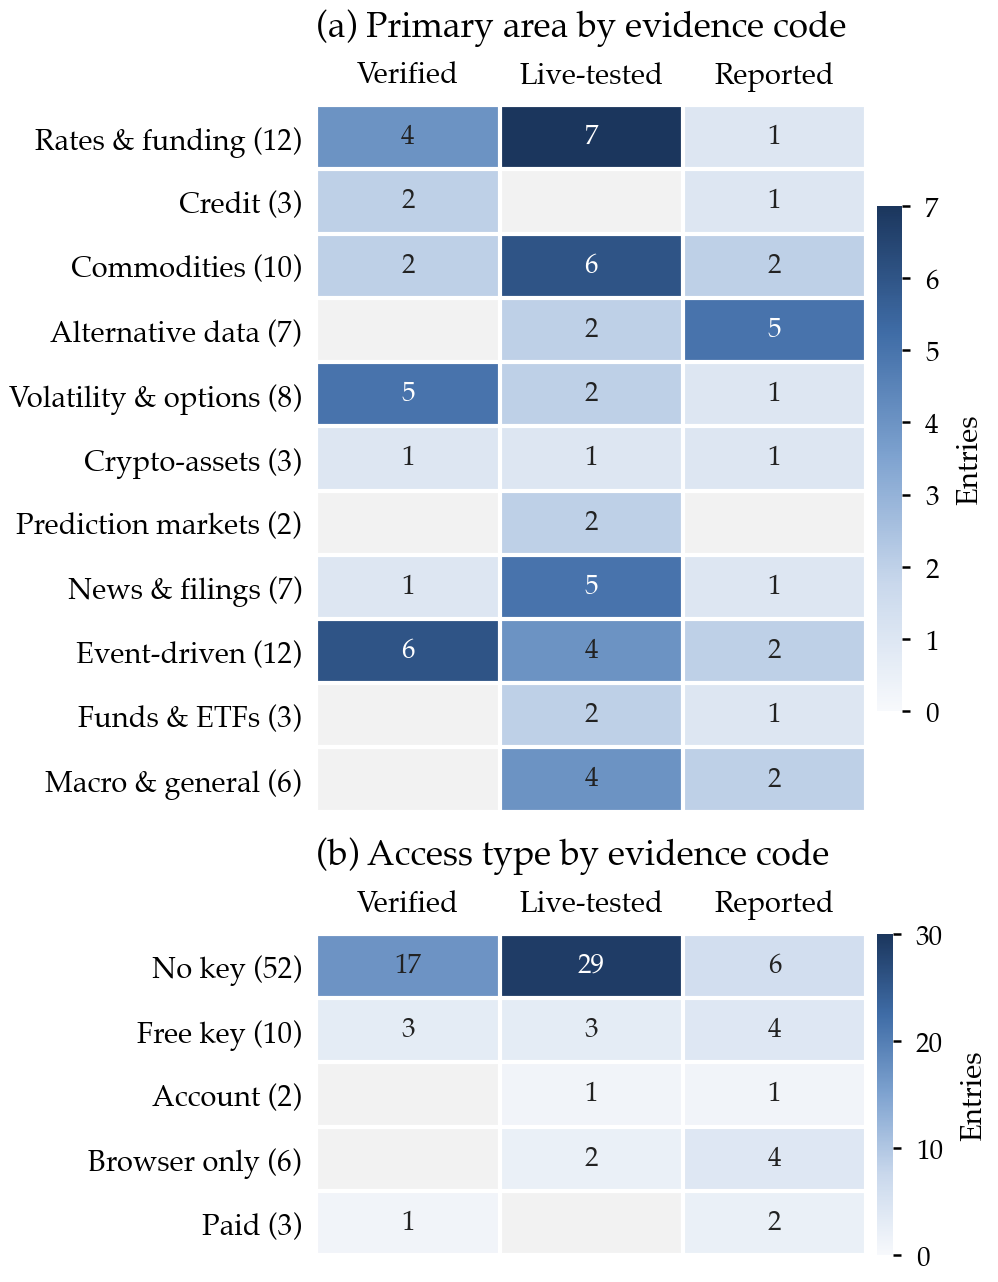
\includegraphics[width=\columnwidth]{figures/evidence_heatmaps.png}
\caption{Catalogue entries by evidence code: (a) by primary area, (b) by access type. Counts of the 73 entries checked on 29 September 2026; row totals in brackets; blank cells are zero.}
\label{fig:evidence}
\qsource{Free-data catalogue, 73 entries checked 29 September 2026; author's tabulation.}
\end{figure}

\subsection{What the counts mean}

The unit of the catalogue is an \emph{entry}, not a provider. A few entries group closely related providers (the IMF, OECD and World Bank interfaces form one entry; so do Reddit and StockTwits, and the press-release feeds of the ECB and the Bank of England), and the SEC appears in five entries because its filing interfaces, full-text search, latest-filings feed, 13F data sets and fails-to-deliver files behave differently. Three paid products (bulk TRACE bond trades, PACER court documents and the former CryptoCompare data service, whose free tier ended on 21 May 2026) are kept because they mark where free access stops. Each entry has a short identifier, shown in the tables, that the playbooks use to refer to it.

%═══════════════════════════════════════════════════════
\section{The Sources by Category}
\label{sec:sources}

The full catalogue, all 73 entries in five groups with what each source provides, its update frequency, the free history, the stated publication timing and the access and evidence codes, is in Appendix~\ref{app:catalogue} (Tables~\ref{tab:src-rates}--\ref{tab:src-macro}). Figure~\ref{fig:attributes} summarises those columns by area: daily data dominate rates, volatility and funds; most filings and event sources update in real time or on release; and the free history is not stated for 51 of the 73 entries.

\begin{figure*}[t]
\centering
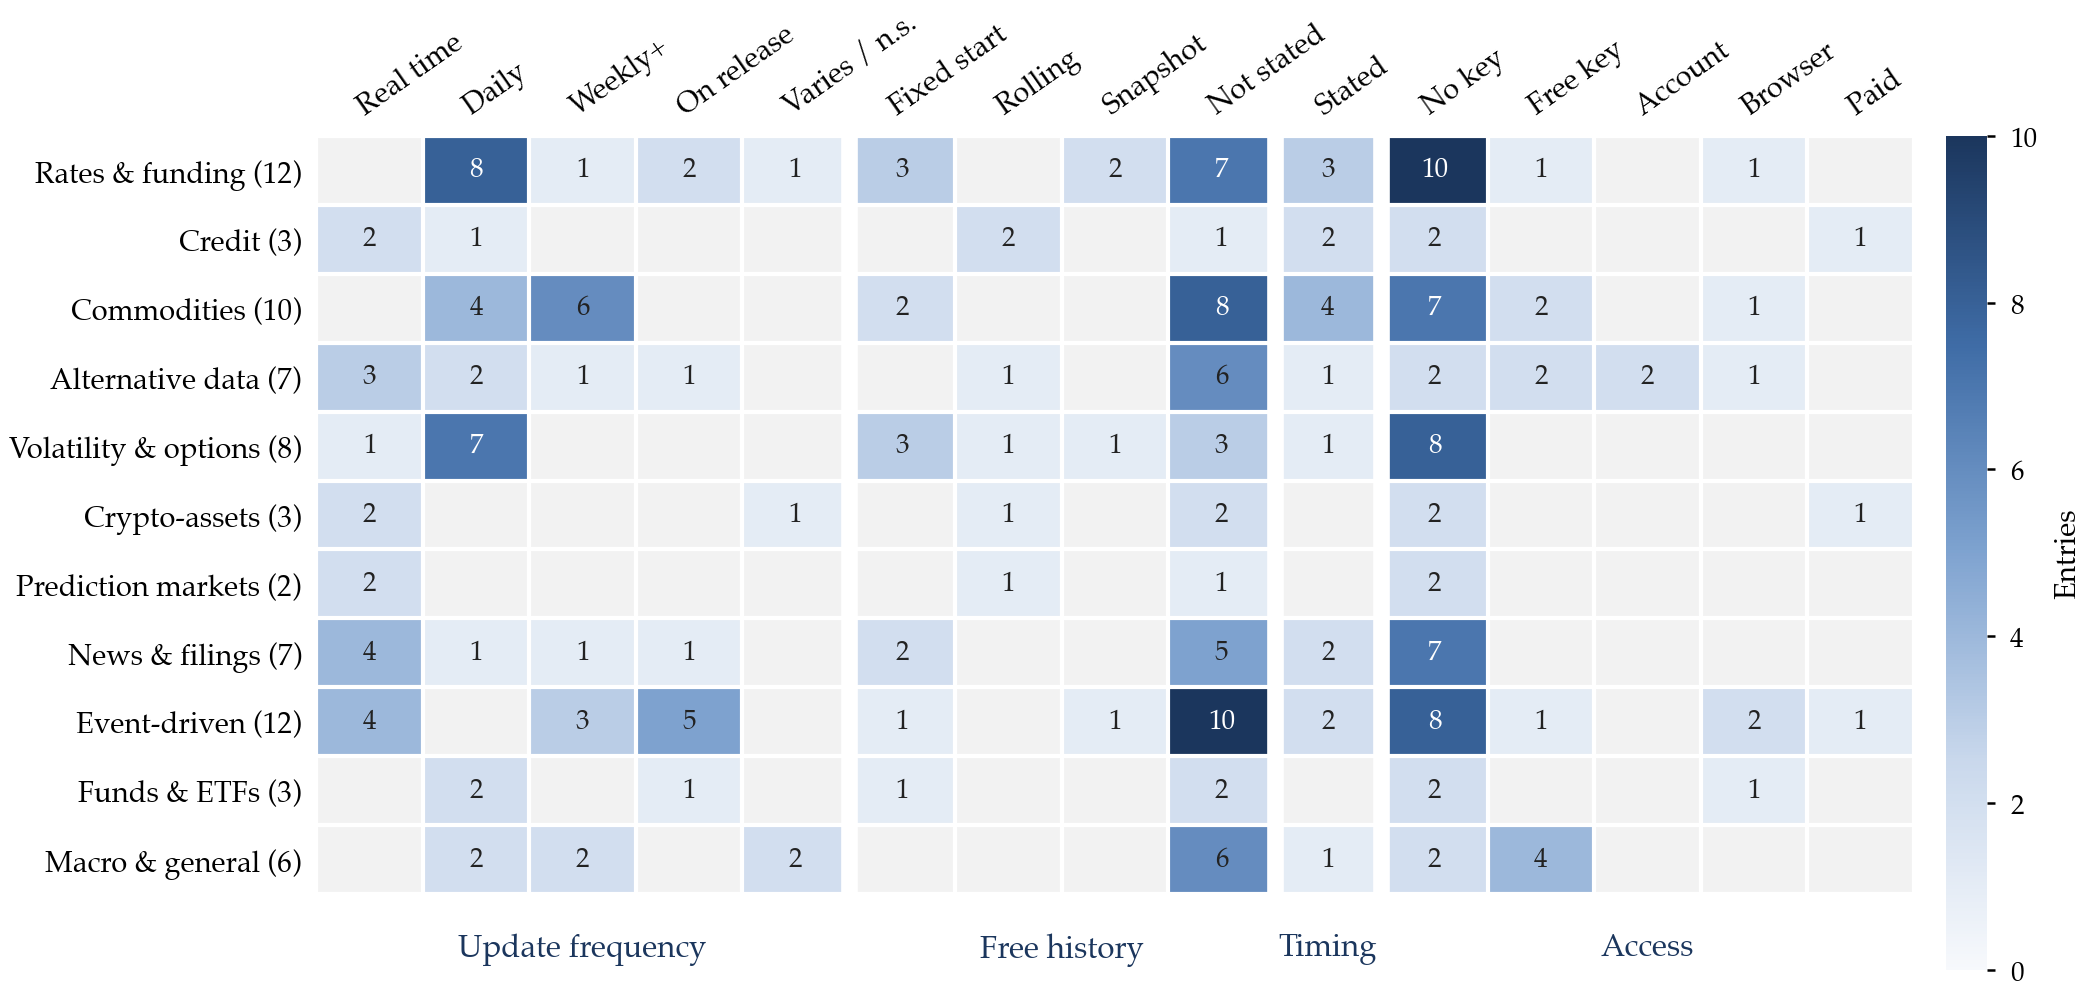
\includegraphics[width=0.94\textwidth]{figures/area_attributes.png}
\caption{Catalogue entries by primary area and attribute: update frequency, free history, whether publication timing is stated, and access type. Counts of the 73 entries checked on 29 September 2026; each attribute group except timing sums to the row total; blank cells are zero. Frequency and history classes are the author's coding of each entry's catalogue fields (``Weekly+'' is weekly or slower).}
\label{fig:attributes}
\qsource{Free-data catalogue, 73 entries checked 29 September 2026; author's tabulation.}
\end{figure*}

\subsection{Rates, funding and credit}

This is the strongest area for free data (Table~\ref{tab:src-rates}). The New York Fed and the OFR \cite{nyfed,ofr} between them publish the secured and unsecured overnight rates with their percentiles and volumes, repo volumes by segment, repo and reverse-repo operations, System Open Market Account (SOMA) holdings, money-fund data and primary-dealer statistics, all without a key. FRED, the St.\ Louis Fed's database, adds ALFRED, which keeps every past vintage of a series \cite{alfred}. The Treasury's FiscalData and TreasuryDirect interfaces \cite{fiscal} give auction results and the Treasury General Account (TGA) balance, and the CFTC's Commitments of Traders (COT) report \cite{cftc} gives weekly positioning in every futures market with enough large traders. Credit is weaker. The ICE BofA option-adjusted spread (OAS) indices on FRED were cut in April 2026 to a rolling three years and carry an internal-use licence; bond trade prints (TRACE) are free only one bond at a time; and municipal data from the MSRB's EMMA was checked only for availability.

\subsection{Commodities, weather and alternative data}

Energy and agriculture are well served by official sources (Table~\ref{tab:src-commod}). The EIA \cite{eia} publishes weekly petroleum and gas storage data both through a keyed API and as plain CSV tables; USDA's National Agricultural Statistics Service (NASS) \cite{usda} publishes crop progress, condition and yields down to county level; and USDA's Foreign Agricultural Service publishes global supply-and-demand balance sheets from 1960. NOAA's Climate Prediction Center publishes population-weighted heating and cooling degree days. Futures prices are the gap: CME settlements, volume and open interest could be viewed in a browser, but scripted requests timed out and bulk history is a paid CME product. The alternative-data entries are mostly R-coded. Only Open-Meteo returned data in a live test; the live test of Reddit and StockTwits found that unauthenticated requests are refused, so registered access is needed.

\subsection{Volatility, options, crypto-assets and prediction markets}

Cboe's public data site \cite{cboe} is the main source of free volatility data (Table~\ref{tab:src-vol}): daily history for VIX and its term-structure siblings, VVIX (the volatility of VIX), SKEW, the COR3M implied-correlation index and commodity volatility indices; per-contract VIX futures files from 2013; and a delayed snapshot of any listed option chain with Cboe-computed implied volatility (IV) and Greeks. The Options Clearing Corporation (OCC) \cite{occ} adds cleared volume split by customer, firm and market maker. What is missing is history of the option chains themselves: the chain is a snapshot, and OCC queries reach back only two years. In crypto-assets, Deribit \cite{deribit} gives option surfaces, a volatility index (DVOL) and funding rates, and Binance gives perpetual-futures funding rates, all without a key. Kalshi and Polymarket \cite{kalshi,poly} publish prices for event contracts on central-bank decisions, data releases and other events.

\subsection{Filings, news, event-driven situations and funds}

The SEC's EDGAR system \cite{sec} is the centre of the event-driven group (Table~\ref{tab:src-event}). Its submission and XBRL financial-statement interfaces are close to real time, and the undocumented full-text search lets a script find new convertible issues, merger proxies, tender offers, spin-off registrations and activist stakes by searching filing text with form and date filters. Around it sit the event calendars a merger-arbitrage or index-rebalance strategy needs: the Federal Trade Commission's (FTC) early-termination notices under the Hart--Scott--Rodino (HSR) Act \cite{ftc}, the UK Competition and Markets Authority's merger cases, federal court dockets through CourtListener \cite{cl}, Delaware bankruptcy claims agents, and index-provider announcements \cite{lseg}. Borrow data is thin: Interactive Brokers' public file gives indicative fees and availability as a current snapshot, and FINRA's short interest is published twice a month \cite{finra}. For funds, CEF Connect gives daily closed-end fund prices, net asset values (NAV) and discounts through an undocumented interface.

\subsection{Macro and general market data}

The last group (Table~\ref{tab:src-macro}) holds the cross-country statistical agencies and the general-purpose market-data services. The Bureau of Labor Statistics (BLS) is notable less for its series than for its calendar: an iCalendar feed of every scheduled release for the year ahead, which is the natural source of availability dates for consumer-price and payroll data. The commercial free tiers change often: Stooq began requiring a key in March 2026, Polygon.io was renamed Massive in October 2025, and the free-tier limits of Alpha Vantage and Massive were not checked.

%═══════════════════════════════════════════════════════
\section{Access Rules}
\label{sec:access}

Free sources impose their own terms, and a pipeline that ignores them fails in ways that range from a blocked address to a breach of licence. Table~\ref{tab:limits} collects the limits and licence terms that the catalogue records. Four rules follow from them.

\emph{Identify and throttle.} EDGAR allows at most ten requests per second across all of a user's machines and requires a User-Agent header naming the requester and a contact address; an address that exceeds the limit is throttled until it has stayed under it for ten minutes. Many other endpoints publish no limit at all, so every caller should throttle by default. Figure~\ref{fig:rates} compares the limits that are stated: they span almost three orders of magnitude.

\begin{figure}[t]
\centering
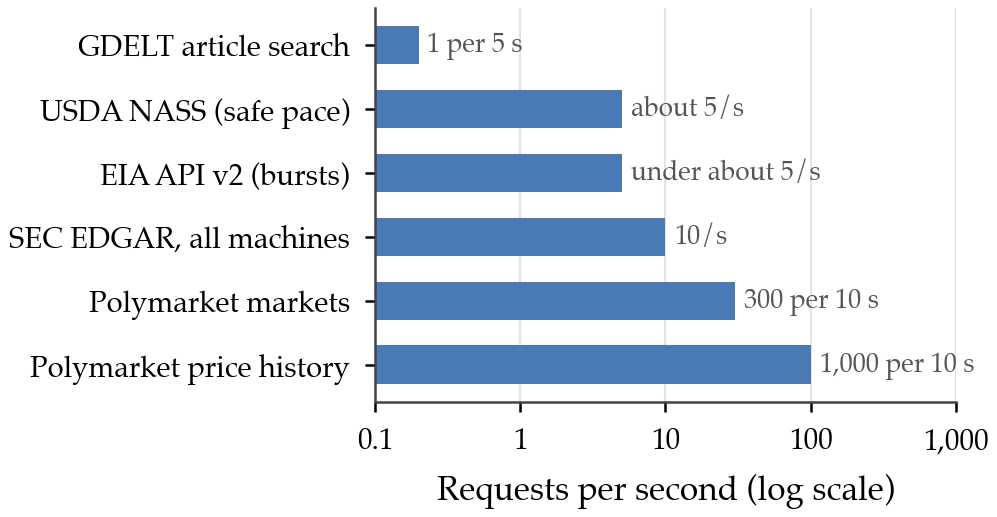
\includegraphics[width=\columnwidth]{figures/rate_limits.png}
\caption{Request limits stated in the catalogue, converted to requests per second (log scale); the stated form is printed beside each bar. Checked 29 September 2026.}
\label{fig:rates}
\qsource{Free-data catalogue, access rules and source entries; author's conversion to a common unit.}
\end{figure}

\emph{Treat undocumented endpoints as fragile.} Six sources (the Cboe option chains and daily statistics, CEF Connect, the Nasdaq calendars, EDGAR full-text search and SqueezeMetrics) are unofficial interfaces behind public web pages. A call to any of them should raise an alert on failure or on a change of schema, rather than write an empty or malformed record. Practical details matter too: Cboe's original data host now redirects to a new one, so a client must follow redirects, and the Nasdaq calendars answer only to a browser-like User-Agent.

\emph{Free to access is not free to redistribute.} The ICE BofA indices on FRED are for internal use only; FINRA data is for non-commercial use; the EIA Daily Prices page republishes third-party prices under licence; and Cboe, the New York Fed, the OCC and SqueezeMetrics each set their own terms. Licences should be checked before any commercial or public use. For this reason the present paper reports no values from these series.

\emph{Re-test before relying on anything.} Every check in the catalogue is a single observation on one date.

\begin{table*}[!t]
\centering
\caption{Access limits and licence terms recorded in the catalogue.}
\label{tab:limits}
\footnotesize
\setlength{\tabcolsep}{3pt}
\qstripes
\begin{tabularx}{\textwidth}{@{}L{1.7cm}Y@{\hspace{14pt}}L{2.1cm}Y@{}}
\toprule
\multicolumn{2}{@{}l}{\qhead{Rate limits and query caps}} & \multicolumn{2}{l@{}}{\qhead{Licence and price terms}} \\
\midrule
SEC EDGAR & 10 requests/s across all machines; User-Agent with name and contact; 10-minute throttle if exceeded & ICE BofA on FRED & No reproduction without permission; internal use only \\
GDELT & Article-search API: 1 request every 5 s & FINRA & Non-commercial use; free TRACE view for personal use \\
USDA NASS & HTTP 429 if too fast (about 5 requests/s is safe); 50,000 records per query & TRACE (paid) & Bulk history \$2,000 set-up plus \$2,000 per extra year; academic \$500 plus \$500 a year, 36-month delay, corporates only, no redistribution \\
EIA API v2 & Bursts under about 5 requests/s; 5,000 rows per response (reported) & EIA & Daily Prices page licensed from Refinitiv, CME, SNL and AAA; API source data public domain \\
Polymarket & 300 requests per 10 s for markets, 1,000 per 10 s for price history; excess delayed, not rejected & PACER (paid) & \$0.10 per page, rising to \$0.12 on 1 January 2027; \$3 cap per document, none on searches \\
FTC & Shared demonstration key runs out after about 3 calls; free key needed & Cboe, NY Fed, OCC, SqueezeMetrics & Each sets its own terms; redistribution terms for the Cboe chains and OCC data not stated or not checked \\
Deribit & Public connections limited to 100 ms aggregation; per-address credit limits & LBMA, Open-Meteo & Check terms before commercial use \\
ALFRED & 110 to 2,000 vintage dates per call, by format & Binance & Check availability in your jurisdiction \\
OCC & Report date no more than 2 years back & & \\
yfinance & Unstated Yahoo rate limits; VPN addresses blocked & & \\
\bottomrule
\end{tabularx}
\qsource{Free-data catalogue, access rules and source entries, checked 29 September 2026.}
\end{table*}

%═══════════════════════════════════════════════════════
\section{Point-in-Time Data and Look-Ahead}
\label{sec:pit}

A backtest is \emph{point-in-time} when every input on a given date is the value that was publicly known on that date. Free sources make this hard in four ways: they publish with a lag that is often unstated; they revise values after first release; they expose only a recent window of history; and their formats change in ways that silently drop data. We take each in turn.

\begin{figure*}[t]
\centering
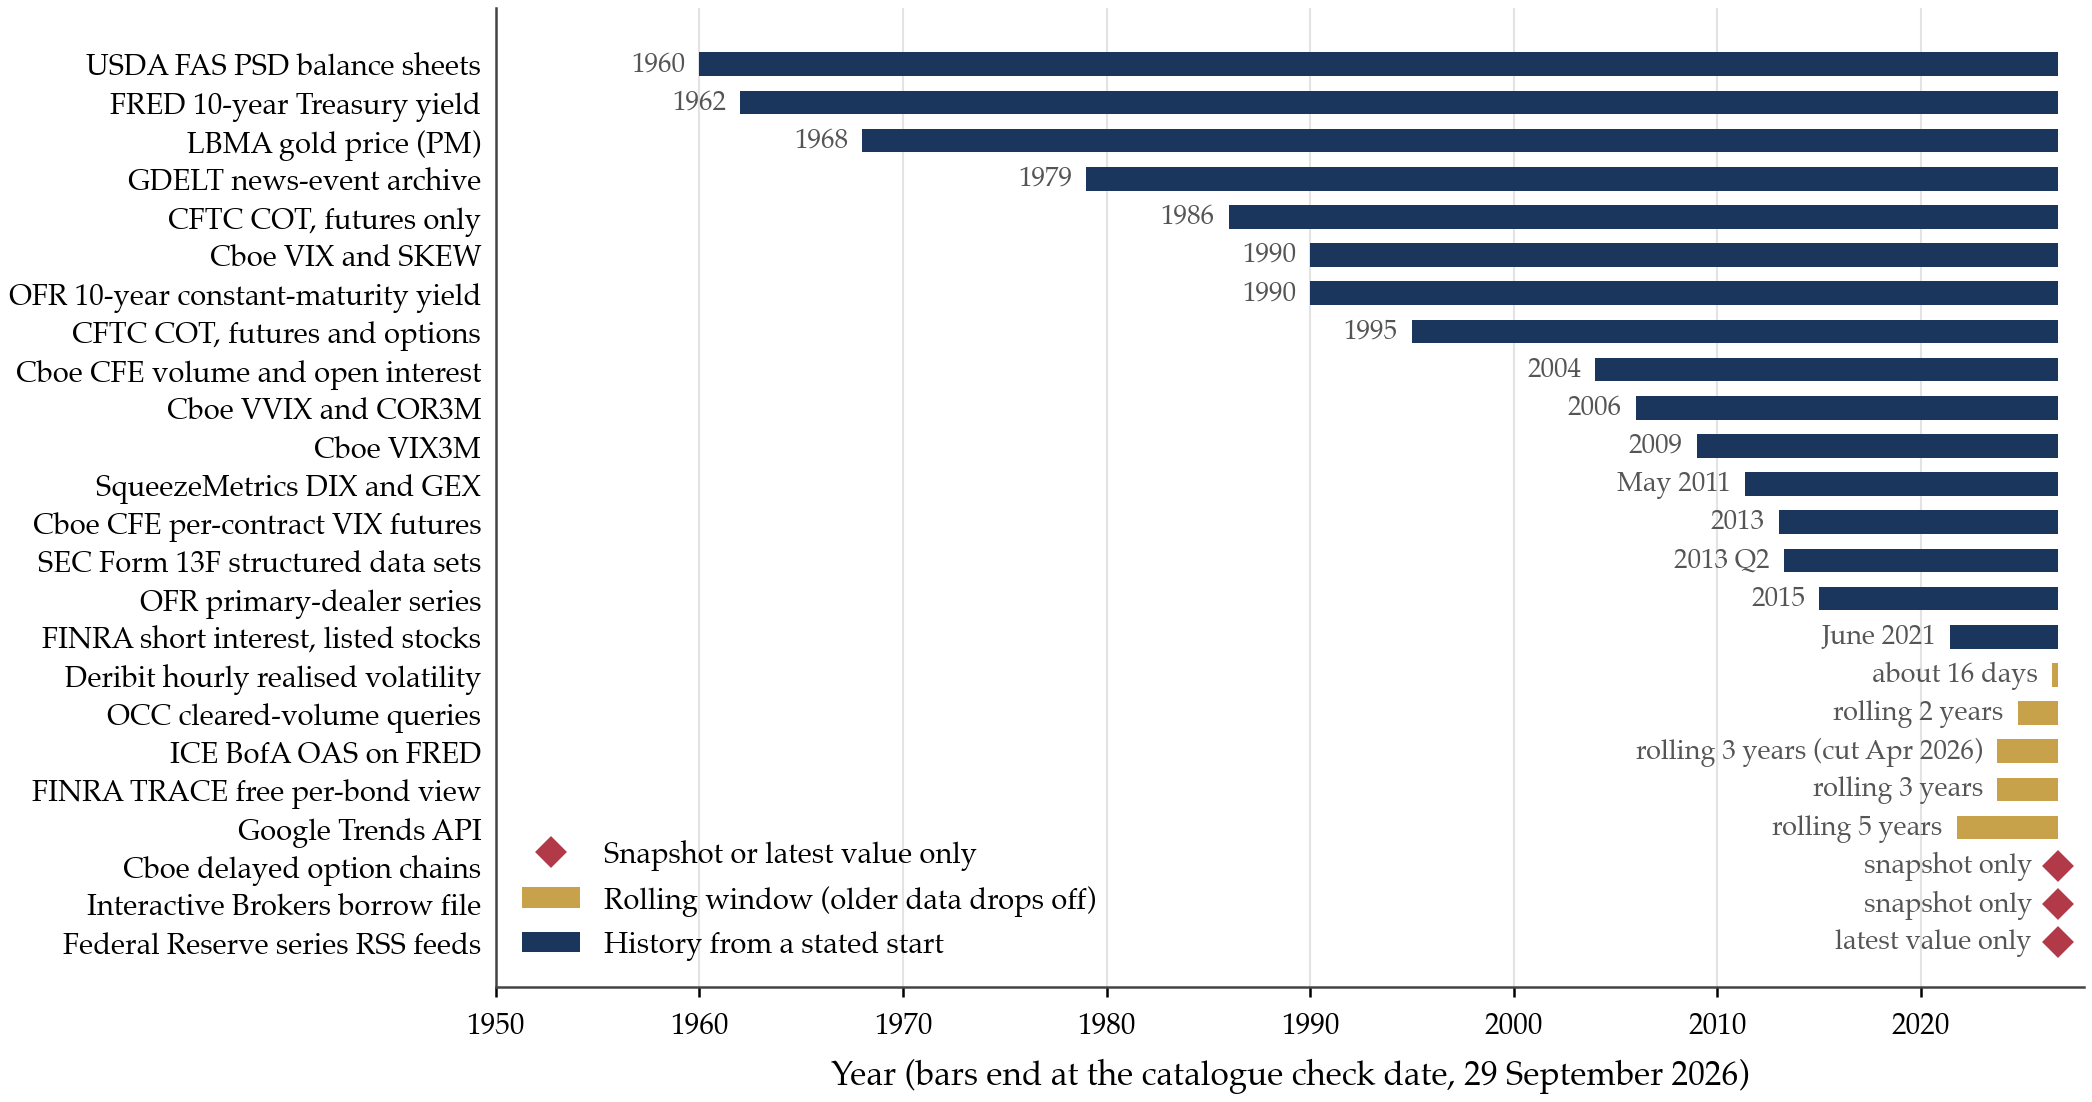
\includegraphics[width=0.84\textwidth]{figures/history_depth.png}
\caption{Free history recorded in the catalogue, by source, to the check date of 29 September 2026. Navy bars start at the stated first year of free history; gold bars are rolling windows whose older data drops off; red diamonds mark sources that expose only a snapshot or the latest value. Sources whose history start is not stated are omitted.}
\label{fig:history}
\qsource{Free-data catalogue, source entries and archive list; author's tabulation.}
\end{figure*}

\subsection{Publication lags}

The date attached to a value is usually the date it describes, not the date it became known. Table~\ref{tab:timing} lists every source for which the catalogue records release timing, with the assumption a backtest must make. The COT report is the standard example: positions are measured on Tuesday and published on Friday at 15:30 ET, so a signal built from a week's positions cannot be dated earlier than the Friday release. Spreads and prices that are posted the next morning (the ICE BofA indices, the EIA price page) belong to the following day. Holdings data sets describe a quarter end that precedes their release. Where the catalogue states no lag, as for FINRA short interest, the lag must be measured before the data are used. Figure~\ref{fig:lags} places the stated delays on one scale: they run from under a second to three years.

\begin{figure}[t]
\centering
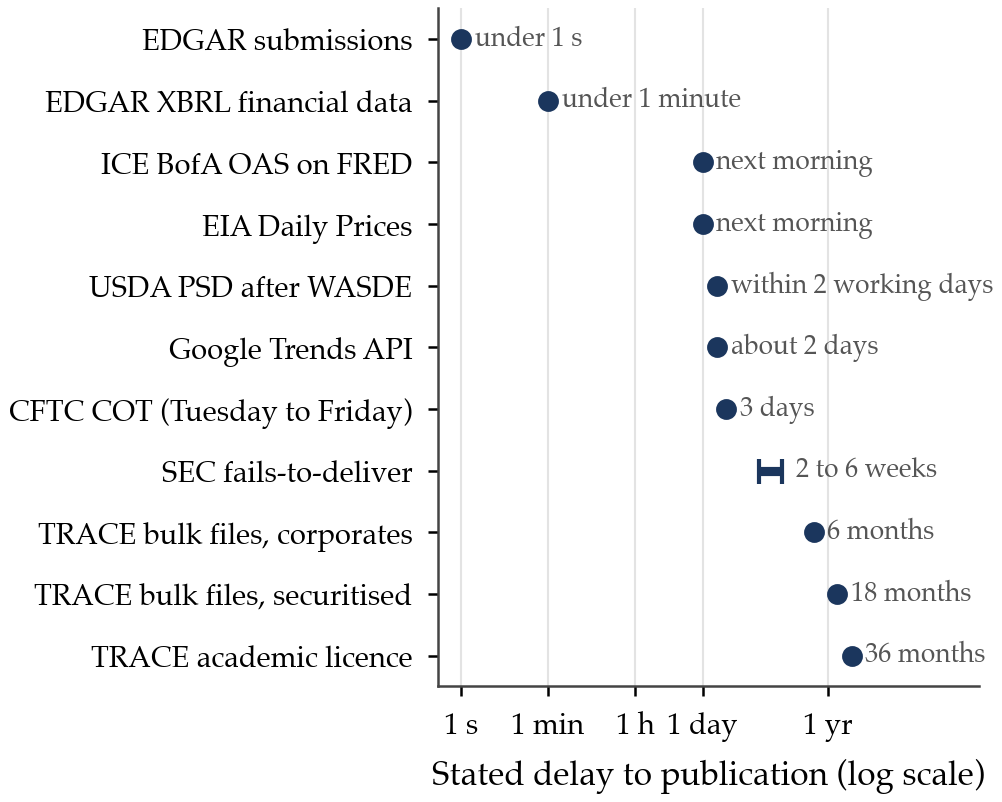
\includegraphics[width=\columnwidth]{figures/publication_lags.png}
\caption{Stated delay between the date a value describes and the date it becomes public, for the entries that state one (log scale). ``Next morning'' is plotted at one day, months at 30.4 days; fails-to-deliver is a 2--6 week range. Checked 29 September 2026.}
\label{fig:lags}
\qsource{Free-data catalogue, source entries; author's conversion to days.}
\end{figure}

\begin{table*}[!t]
\centering
\caption{Publication timing recorded in the catalogue, and the assumption a point-in-time backtest must make.}
\label{tab:timing}
\footnotesize
\setlength{\tabcolsep}{4pt}
\qstripes
\begin{tabularx}{\textwidth}{@{}L{3.4cm}L{6.4cm}Y@{}}
\toprule
\qhead{Source} & \qhead{When a value becomes public (catalogue)} & \qhead{Assumption for a backtest} \\
\midrule
CFTC COT & Positions as of Tuesday; released Friday 15:30 ET & A week's positions are usable only from the Friday release \\
ICE BofA OAS on FRED & Daily close, posted the next morning & The spread for day $t$ is known on day $t+1$ \\
EIA Daily Prices & Weekdays about 07:30--08:30 ET, using prior-day closes & Prices for day $t$ are known on the morning of day $t+1$ \\
EIA API v2 & No ``last updated'' field in the interface & Availability dates must come from EIA's release calendar, kept separately \\
FRED / ALFRED & Every past vintage kept; first prints differ from revised values & Use the vintage in force on the decision date, never the latest value \\
BLS & Calendar of scheduled release times for the year ahead & Date each print by its scheduled release time \\
Federal Reserve Board RSS & Time stamp is the scheduled release time; newswires can be faster & The feed's time stamp is not an arrival time in live use \\
USDA FAS PSD & Updated within 2 working days of the WASDE report & The news was public at the WASDE release; dating it by the PSD update is late but safe \\
SEC fails-to-deliver & Twice monthly, 2--6 weeks after the fact & Date records by publication, never by settlement date \\
FINRA short interest & Twice monthly; publication lag not stated & Measure the lag before use \\
SEC Form 13F data sets & Quarterly; released after the end of February, May, August and November & Holdings describe an earlier quarter end; date them by release or filing \\
SEC EDGAR & Submissions within 1 s, XBRL within 1 minute & Date a filing signal by when the filing became public, not by the period it covers \\
Google Trends API & Data up to about 2 days ago & Allow at least a 2-day lag \\
UN Comtrade & Monthly, lagged by country & No single lag applies; record availability by reporter \\
FTSE Russell & For December 2026: rank day 30 Oct, preliminary lists 13 Nov, lock-down 30 Nov, effective after the close on 11 Dec & Date a membership change by its list publication, not its effective date \\
Cboe chains; IBKR borrow file & Delayed snapshot (cached about 5 s); borrow file updated through the day & Store the retrieval time with every capture \\
\bottomrule
\end{tabularx}
\qsource{Free-data catalogue, source entries; the right-hand column is the author's reading of each timing rule.}
\end{table*}

\subsection{Revisions and vintages}

Macroeconomic data are revised after first release, and a backtest that uses today's revised series is using numbers no one had at the time \cite{croushore2001}. ALFRED solves this for FRED series by keeping every vintage, so a series can be read as it stood on any past date; the OFR's interface also offers vintage selection. A macro-surprise model should pair ALFRED's first prints with the BLS release calendar for timing. Two caveats from the catalogue apply: ALFRED caps each call at between 110 and 2,000 vintage dates depending on format, and since January 2026 FRED user accounts can no longer save ALFRED data, although interface access to vintages is unaffected. For a source that keeps no vintages, the only point-in-time record is one the desk keeps itself.

\subsection{Truncated, rolling and snapshot history}

Figure~\ref{fig:history} shows the free history the catalogue records for each source that states one. Long histories (USDA balance sheets from 1960, the 10-year Treasury yield from 1962, the COT report from 1986, VIX from 1990) sit beside sources whose history moves: the ICE BofA spread indices on FRED keep only three years, OCC volume queries two, and Deribit's hourly realised volatility about sixteen days. Snapshot sources keep none. For these sources a backtest can begin only on the day an archive began, and any statistic computed before that day must come from another source. A related trap is silent loss: Kalshi moves data older than a rolling cutoff to separate historical endpoints, and a pipeline that queries only the live endpoints loses history without any error.

\subsection{Schema breaks and silent truncation}

The most dangerous failures raise no error. Table~\ref{tab:breaks} lists the format changes and quirks the catalogue records. The CFTC case shows the pattern: Treasury futures were renamed around February 2022 (for example to ``UST 10Y NOTE''), so a query that filters on a contract name containing ``TREASURY'' returns a series that simply stops in 2022. Filtering by the CFTC contract code avoids it. Similarly, an EDGAR full-text query for the old form code ``SC 13D'' returned nothing for late September 2026, because ownership filings now use ``SCHEDULE 13D''.

\begin{table*}[!t]
\centering
\caption{Format changes and data quirks recorded in the catalogue.}
\label{tab:breaks}
\footnotesize
\setlength{\tabcolsep}{3pt}
\qstripes
\begin{tabularx}{\textwidth}{@{}L{1.7cm}Y@{\hspace{14pt}}L{1.7cm}Y@{}}
\toprule
\qhead{Source} & \qhead{Break or quirk} & \qhead{Source} & \qhead{Break or quirk} \\
\midrule
CFTC COT & Contract names changed around Feb 2022; name filters stop silently. Filter by contract code & Cboe chains & Deep in-the-money and illiquid strikes show IV of 0 \\
EDGAR search & Ownership filings use ``SCHEDULE 13D/13G''; ``SC 13D'' returns nothing & FINRA SI & Pipe-delimited despite a .csv name; before June 2021, OTC stocks only \\
NY Fed & EFFR before 2016 uses a different schema; SOFR averages carry no percentiles & SEC FTD & Before September 2008, only fails of 10,000 shares or more \\
Cboe CFE & Settlement is 0 before May 2013 (use the close); one file per expiry; the volume file has a disclaimer row, duplicate column names and a misspelled header & USDA NASS & County figures may not sum to state totals \\
Cboe indices & Early VIX rows are close-only; 2006 VVIX rows are sparse and dirty & ETF holdings & Formats differ by issuer; one issuer's CSV link returned a web page \\
ICE BofA & Cut to a rolling 3 years in April 2026; series now start 30 Sep 2023 & GDELT & Machine-coded; expect duplicates and obscure sources \\
FTSE Russell & Russell U.S.\ indexes now reconstitute in June and December & & \\
\bottomrule
\end{tabularx}
\qsource{Free-data catalogue, source entries and changes timeline, checked 29 September 2026.}
\end{table*}

\subsection{Estimated and single-vendor series}

Some free series are model outputs rather than observations. SqueezeMetrics' GEX is an estimate of dealer gamma exposure from one private vendor, with no licence or service guarantee, at a web address that could change. Cboe's chain carries Cboe's own IV and Greeks, which depend on Cboe's model inputs; GDELT's events are machine-coded. Such series can be useful filters, but a backtest that uses them inherits the vendor's method, and any later change to that method changes the history without notice.

%═══════════════════════════════════════════════════════
\section{Strategy Playbooks}
\label{sec:playbooks}

The catalogue maps 33 strategy playbooks, in six groups, to the sources that supply their inputs (Figure~\ref{fig:matrix}) and to what probably has to be bought (Table~\ref{tab:playbooks}).

\begin{figure*}[t]
\centering
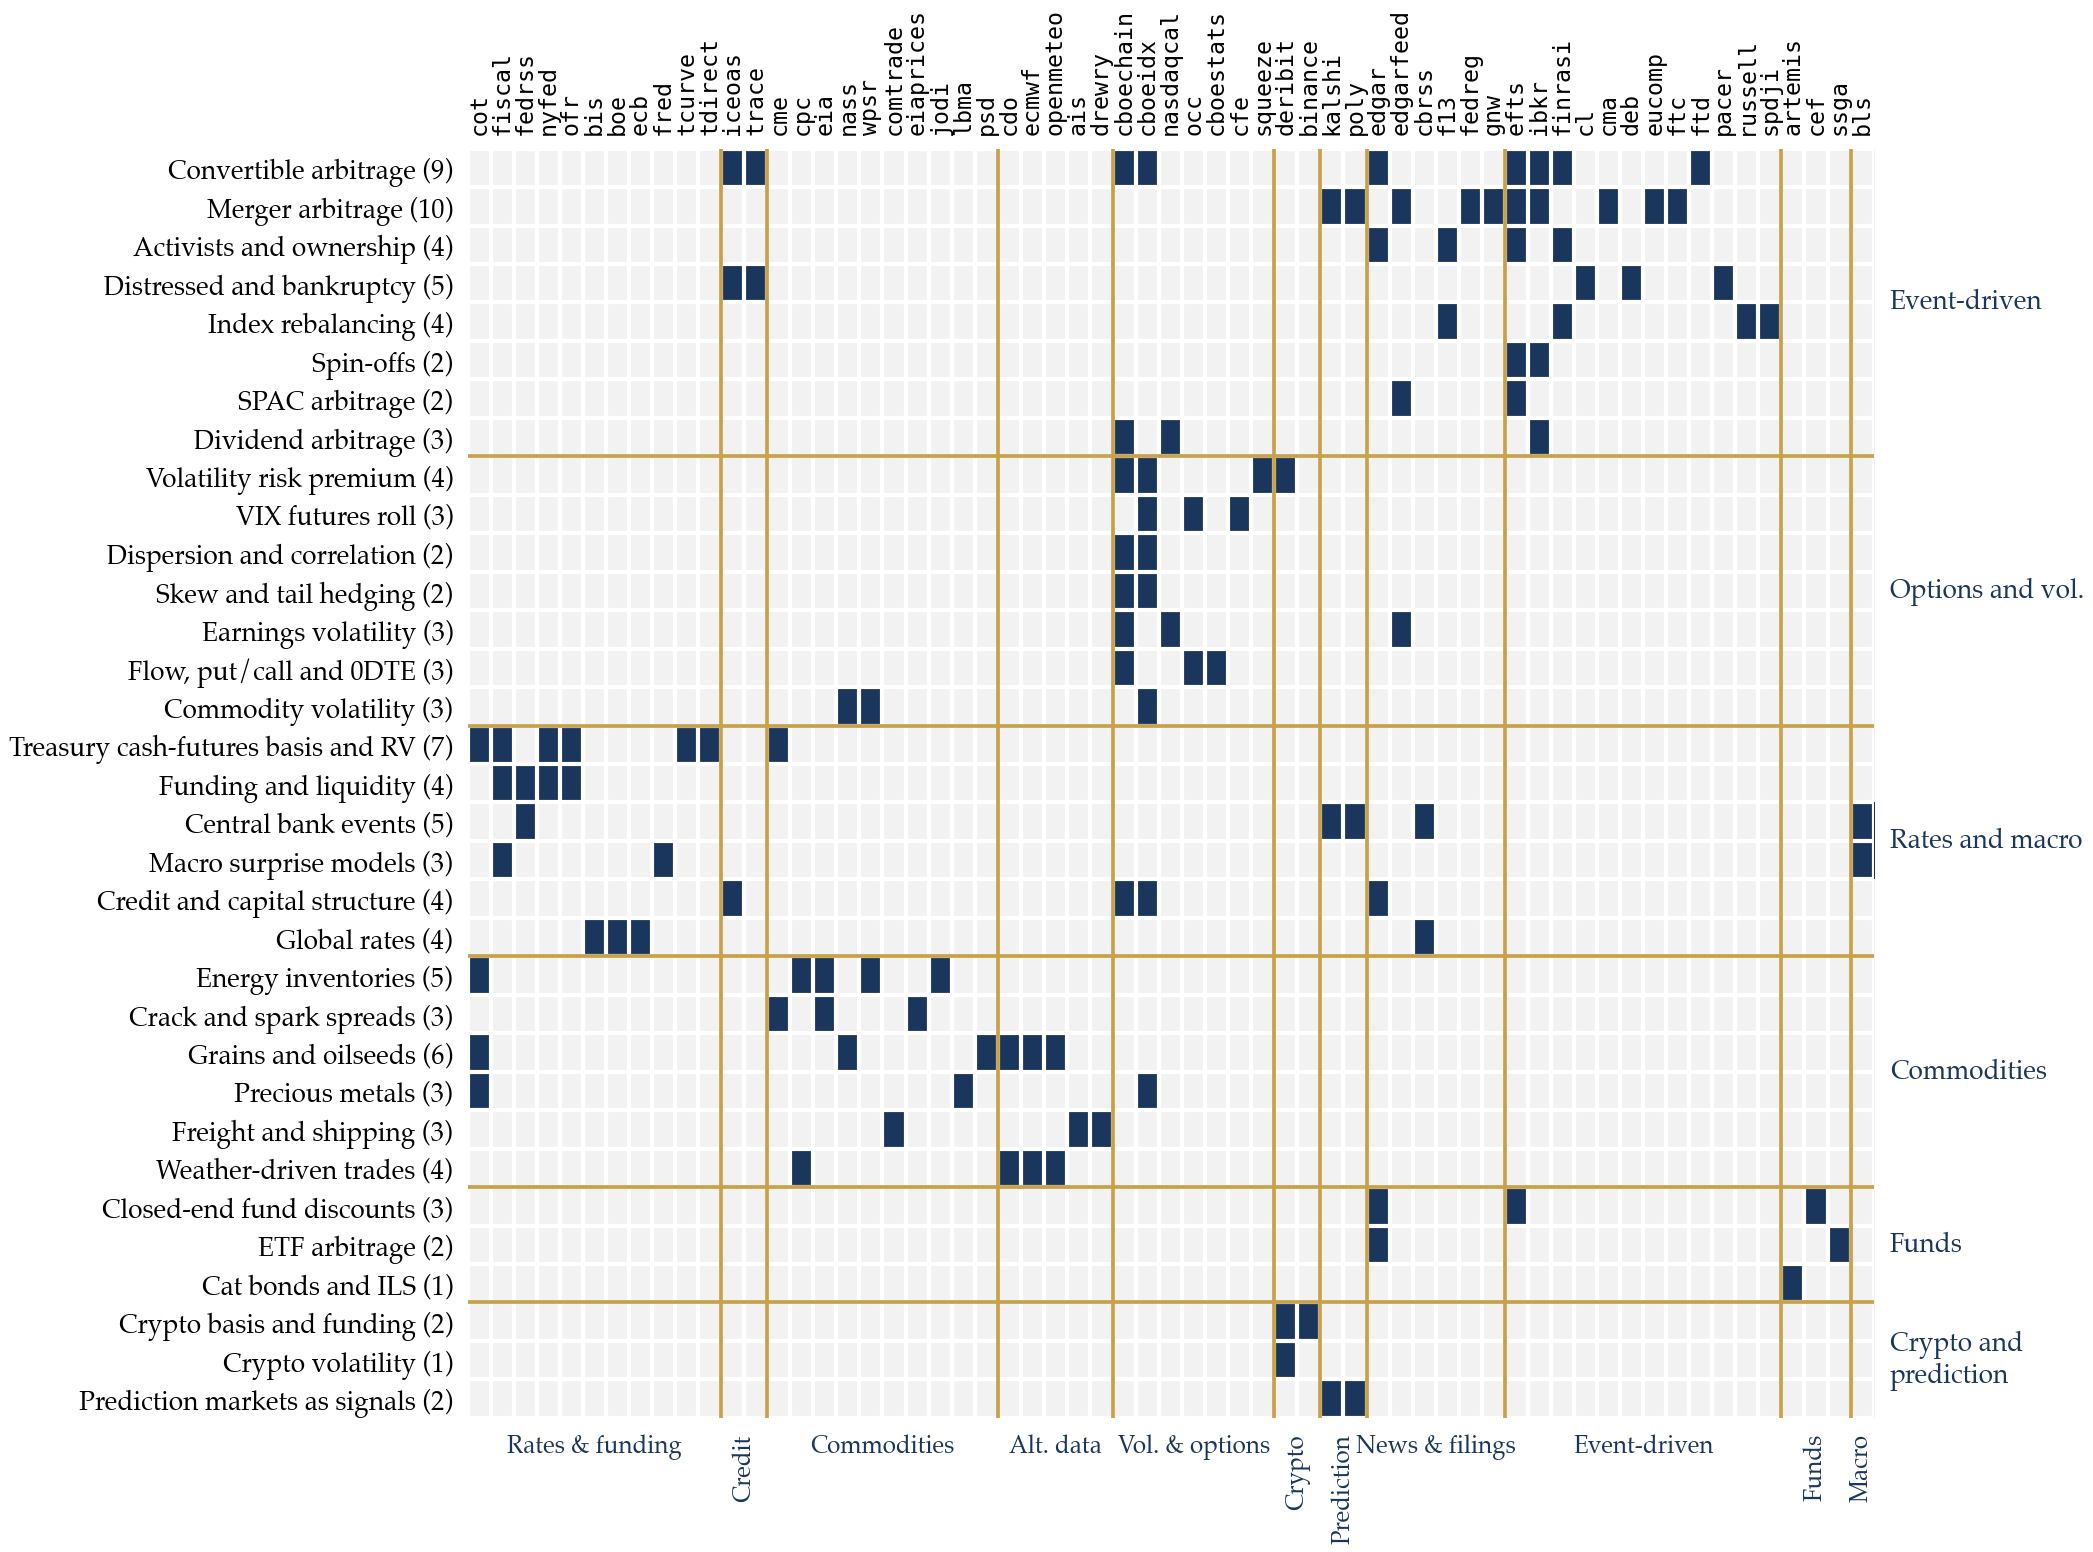
\includegraphics[width=\textwidth]{figures/playbook_matrix.png}
\caption{Which free sources each playbook uses. Rows are the 33 playbooks, grouped as in the catalogue, with the number of free inputs in brackets; columns are the 61 entries named by at least one playbook, grouped by primary area; a filled cell means the playbook names the entry as an input. Entries named only as a warning (the retired CryptoCompare tier) or by no playbook are omitted. Catalogue checked 29 September 2026.}
\label{fig:matrix}
\qsource{Free-data catalogue, strategy playbooks and source index; author's tabulation.}
\end{figure*} A playbook is a list of inputs, not a tested strategy: it says what a strategy of that kind needs and where to get it, and makes no claim that the strategy is profitable.

\begin{table*}[!t]
\centering
\caption{What each of the 33 playbooks has to buy, or cannot find free, as recorded in the catalogue. The free inputs of each playbook are shown in Figure~\ref{fig:matrix}.}
\label{tab:playbooks}
\footnotesize
\setlength{\tabcolsep}{3.5pt}
\qstripes
\begin{tabularx}{\textwidth}{@{}L{3.6cm}Y@{\hspace{12pt}}L{3.6cm}Y@{}}
\toprule
\qhead{Playbook} & \qhead{Paid or missing} & \qhead{Playbook} & \qhead{Paid or missing} \\
\midrule
\multicolumn{2}{@{}l}{\textit{Event-driven and arbitrage}} & \multicolumn{2}{l@{}}{\textit{Rates and macro}} \\
Convertible arbitrage & Terms database, new-issue calendar, bulk TRACE, CDS, live borrow & Treasury basis and relative value & CME settlement history, CTD and conversion factors, bond prices \\
Merger arbitrage & Curated spread database; HSR second requests; China SAMR & Funding and liquidity & Nothing essential \\
Activists and ownership & Nothing essential & Central-bank events & Low-latency newswire \\
Distressed and bankruptcy & Claims-trading data, bulk bond prints & Macro surprise models & Consensus forecast history \\
Index rebalancing & Pro-forma constituent files & Credit and capital structure & CDS, bulk TRACE, long OAS history \\
Spin-offs & Nothing essential & Global rates & Swap curves beyond a few points \\
SPAC arbitrage & Structured SPAC tracker & \multicolumn{2}{l@{}}{\textit{Commodities}} \\
Dividend arbitrage & Real-time borrow, dividend forecasts & Energy inventories & Tank-level or satellite storage data \\
\multicolumn{2}{@{}l}{\textit{Options and volatility}} & Crack and spark spreads & Futures curve history \\
Volatility risk premium & IV surfaces before the archive starts & Grains and oilseeds & Satellite crop imagery \\
VIX futures roll & Nothing essential & Precious metals & Vault and ETF flow detail \\
Dispersion and correlation & Single-stock IV surface history & Freight and shipping & Baltic indices, FFA curves (not checked) \\
Skew and tail hedging & Skew surface history & Weather-driven trades & Ensemble forecast archives \\
Earnings volatility & IV history around past earnings & \multicolumn{2}{l@{}}{\textit{Crypto-assets and prediction markets}} \\
Flow, put/call and 0DTE & Intraday OPRA tape & Basis and funding & Consolidated multi-exchange data \\
Commodity volatility & CME options surfaces & Crypto volatility & Long realised-volatility history \\
\multicolumn{2}{@{}l}{\textit{Funds and structure}} & Prediction markets as signals & Nothing essential \\
Closed-end fund discounts & Nothing essential &  &  \\
ETF arbitrage & Intraday indicative NAV &  &  \\
Catastrophe bonds and ILS & Secondary pricing and index data &  &  \\
\bottomrule
\end{tabularx}
\qsource{Free-data catalogue, strategy playbooks (33), checked 29 September 2026.}
\end{table*}

\subsection{Which sources carry the most strategies}

Counting how many playbooks name each source as an input gives a rough measure of where free data is most valuable (Figure~\ref{fig:cites}). Two Cboe feeds, the volatility-index history and the delayed option chains, each support eight of the 33 playbooks; EDGAR full-text search supports six and the EDGAR interfaces five; the Interactive Brokers borrow file and the COT report four each. In all, 61 of the 73 entries are named as an input by at least one playbook. The former CryptoCompare service is named only as a warning that its free tier has gone, and 11 entries are named by none: the international statistics interfaces, the Chatham rates page, EMMA, yfinance, GDELT, Google Trends, the social-media interfaces and the four general-purpose market-data services. These may still be useful; they are simply not the first choice for any listed strategy.

\begin{figure}[t]
\centering
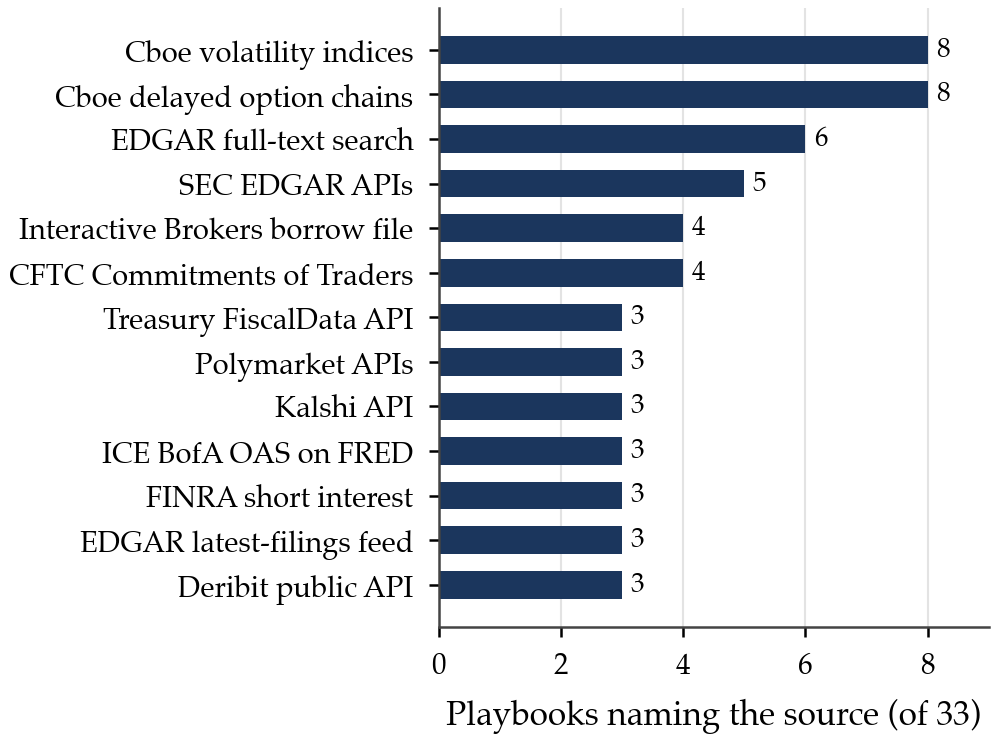
\includegraphics[width=\columnwidth]{figures/playbook_citations.png}
\caption{Sources named as an input by three or more of the 33 playbooks (column totals of Figure~\ref{fig:matrix}). A further 17 entries are named by two playbooks and 31 by one. Catalogue checked 29 September 2026.}
\label{fig:cites}
\qsource{Free-data catalogue, 73 entries checked 29 September 2026; author's tabulation.}
\end{figure}

The pattern matters for priorities. Option chains and borrow availability both appear near the top, and both are snapshot sources: the two inputs that support the most strategies are among those whose history is lost if it is not captured. Free data is rarely the whole answer, however. Only 6 of the 33 playbooks record nothing essential to buy (Figure~\ref{fig:suff}); every commodity playbook needs at least one paid or missing input.

\begin{figure}[t]
\centering
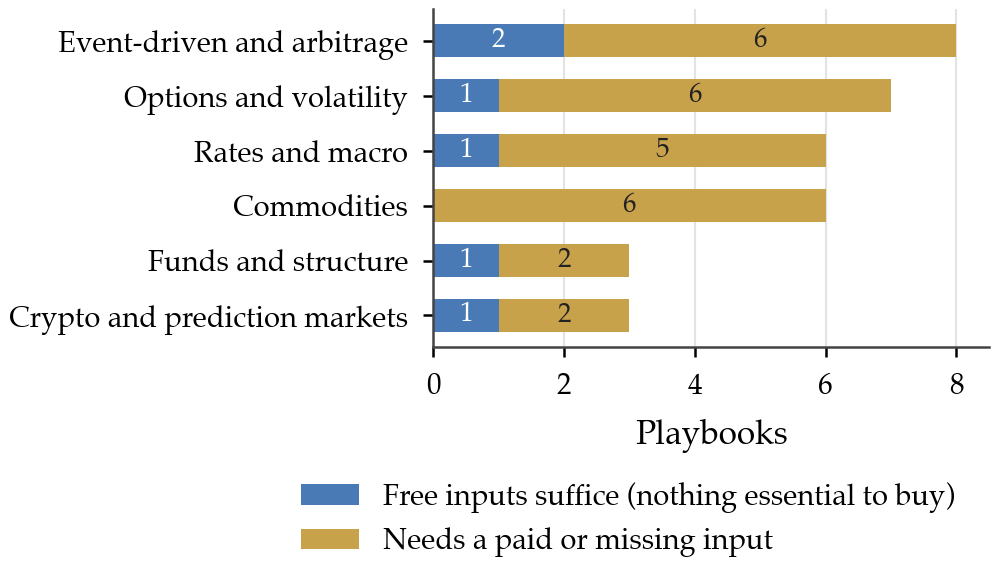
\includegraphics[width=\columnwidth]{figures/playbook_sufficiency.png}
\caption{Playbooks by group, split by whether the catalogue records ``nothing essential'' to buy or a paid or missing input. Counts of the 33 playbooks; catalogue checked 29 September 2026.}
\label{fig:suff}
\qsource{Free-data catalogue, strategy playbooks; author's tabulation.}
\end{figure}

\subsection{Twelve priority feeds}

If only a few feeds can be built, the survey recommends twelve, covering 23 catalogue entries: funding rates and repo (\sid{nyfed}, \sid{ofr}); Treasury auctions, the TGA and the curve (\sid{fiscal}, \sid{tdirect}, \sid{tcurve}); macro vintages (\sid{fred}); futures positioning (\sid{cot}); energy stocks (\sid{eia}, \sid{wpsr}); crop condition and global balance sheets (\sid{nass}, \sid{psd}); volatility indices and VIX futures (\sid{cboeidx}, \sid{cfe}); option chains and cleared volume (\sid{cboechain}, \sid{occ}); filings (\sid{edgar}, \sid{efts}); borrow and short interest (\sid{ibkr}, \sid{finrasi}); crypto option surfaces and funding (\sid{deribit}, \sid{binance}); and event odds (\sid{kalshi}, \sid{poly}). All are free, can be scripted, and returned data on 29 September 2026.

%═══════════════════════════════════════════════════════
\section{Where Free Data Runs Out}
\label{sec:gaps}

Table~\ref{tab:gaps} lists the needs for which no usable free source was found, with the best free substitute and how far each was checked, from verified to not checked. The catalogue's summary names six purchases: bulk TRACE history, historical implied-volatility surfaces, a convertible-terms database, CDS spreads, live borrow, and CME settlement history.

\begin{table*}[!t]
\centering
\caption{Needs with no usable free source. Status records how far each row was checked.}
\label{tab:gaps}
\footnotesize
\setlength{\tabcolsep}{4pt}
\qstripes
\begin{tabularx}{\textwidth}{@{}L{4.2cm}L{5.2cm}Y@{}}
\toprule
\qhead{Need} & \qhead{Best free substitute} & \qhead{Status} \\
\midrule
Bulk historical bond trades (TRACE) & Per-bond free site (\sid{trace}) & V: bulk history \$2,000 set-up plus \$2,000 per extra year; academic \$500 plus \$500 a year, 36-month delay, corporates only \\
Historical option chains and IV surfaces & Start archiving \sid{cboechain} now & V: free sources are snapshots; \sid{occ} has volume and open interest only \\
Convertible terms and new-issue calendar & Parse the pricing 8-K and the indenture filed with the closing 8-K (\sid{efts}) & V: no free bulk source; most new converts are Rule 144A deals with no 424B prospectus \\
Live borrow rates and locates & Indicative public file (\sid{ibkr}) & V: the full securities-lending tool needs a brokerage account \\
CME futures and options settlement history & Browser view (\sid{cme}); \sid{cot} for positioning & L: scripted requests timed out; bulk history is paid \\
CDS spreads & \sid{iceoas} as a proxy & Not found \\
Curated merger-arbitrage spread tracker & Build from \sid{efts} deal terms plus prices & Not found \\
SPAC trust values and redemption deadlines & \sid{efts} filings & Not found \\
Intraday options tape (OPRA) & \sid{cboechain}, \sid{occ} & Not checked \\
Baltic freight indices and FFA curves & \sid{ais}, \sid{drewry}, \sid{comtrade} & Not checked \\
China SAMR merger reviews, machine-readable & None identified & Not checked \\
\bottomrule
\end{tabularx}
\qsource{Free-data catalogue, gaps table, checked 29 September 2026.}
\end{table*}

The convertible-bond row illustrates how far free filings can go. In a verified example from January 2026, the pricing 8-K (Item 8.01) gave the size, coupon, maturity, initial conversion rate (62.5626 shares per \$1,000 principal, a conversion price of about \$15.98), the conversion premium and the capped-call terms; the closing 8-K filed the indenture and the form of note as exhibits, which hold the call, put and make-whole schedules. A terms database can therefore be built from filings, at the cost of parsing every new issue's filings.

The survey also lists areas it did not research in depth, where absence from the catalogue says nothing about quality: the X (Twitter) interface, satellite imagery, job postings, patents, EU and Chinese merger dockets beyond availability, Baltic freight, catastrophe-bond pricing, CDS and economic consensus forecasts.

%═══════════════════════════════════════════════════════
\section{What to Archive, and Why}
\label{sec:archive}

Because several of the best free sources are snapshots or rolling windows, the survey names a daily archiver as the highest-value build task. Table~\ref{tab:archive} gives the archive list. Each row is a source whose history cannot be recovered later for free.

\begin{table*}[!t]
\centering
\caption{Sources to store on a schedule: the free window, what to keep, and the suggested cadence.}
\label{tab:archive}
\footnotesize
\setlength{\tabcolsep}{4pt}
\qstripes
\begin{tabularx}{\textwidth}{@{}L{3.6cm}YL{3.6cm}L{3.2cm}@{}}
\toprule
\qhead{Source} & \qhead{What to store} & \qhead{Free window} & \qhead{Cadence} \\
\midrule
Cboe delayed option chains & Per-strike IV, Greeks, open interest and quotes for SPX, SPY, VIX and target single names & Snapshot only & Daily after the close \\
OCC market data & Volume by account type (customer, firm, market maker), puts and calls & Rolling 2 years & Daily \\
ICE BofA OAS on FRED & High-yield, BBB, investment-grade and AAA spreads & Rolling 3 years (since April 2026) & Daily \\
Interactive Brokers shortable file & Borrow fee, rebate, shares available & Snapshot only & Several times a day \\
Deribit & Hourly realised volatility & About 16 days & Weekly \\
Federal Reserve Board RSS & H.15 and H.10 series values & Latest value only & Daily, or use FRED for history \\
FINRA TRACE free site & Trade prints for the bonds followed & Rolling 3 years & As needed \\
Kalshi & Markets, trades, candlesticks & Live endpoints drop data older than a rolling cutoff & Query live and historical endpoints and merge \\
\bottomrule
\end{tabularx}
\qsource{Free-data catalogue, archive list, checked 29 September 2026.}
\end{table*}

\begin{figure*}[t]
\centering
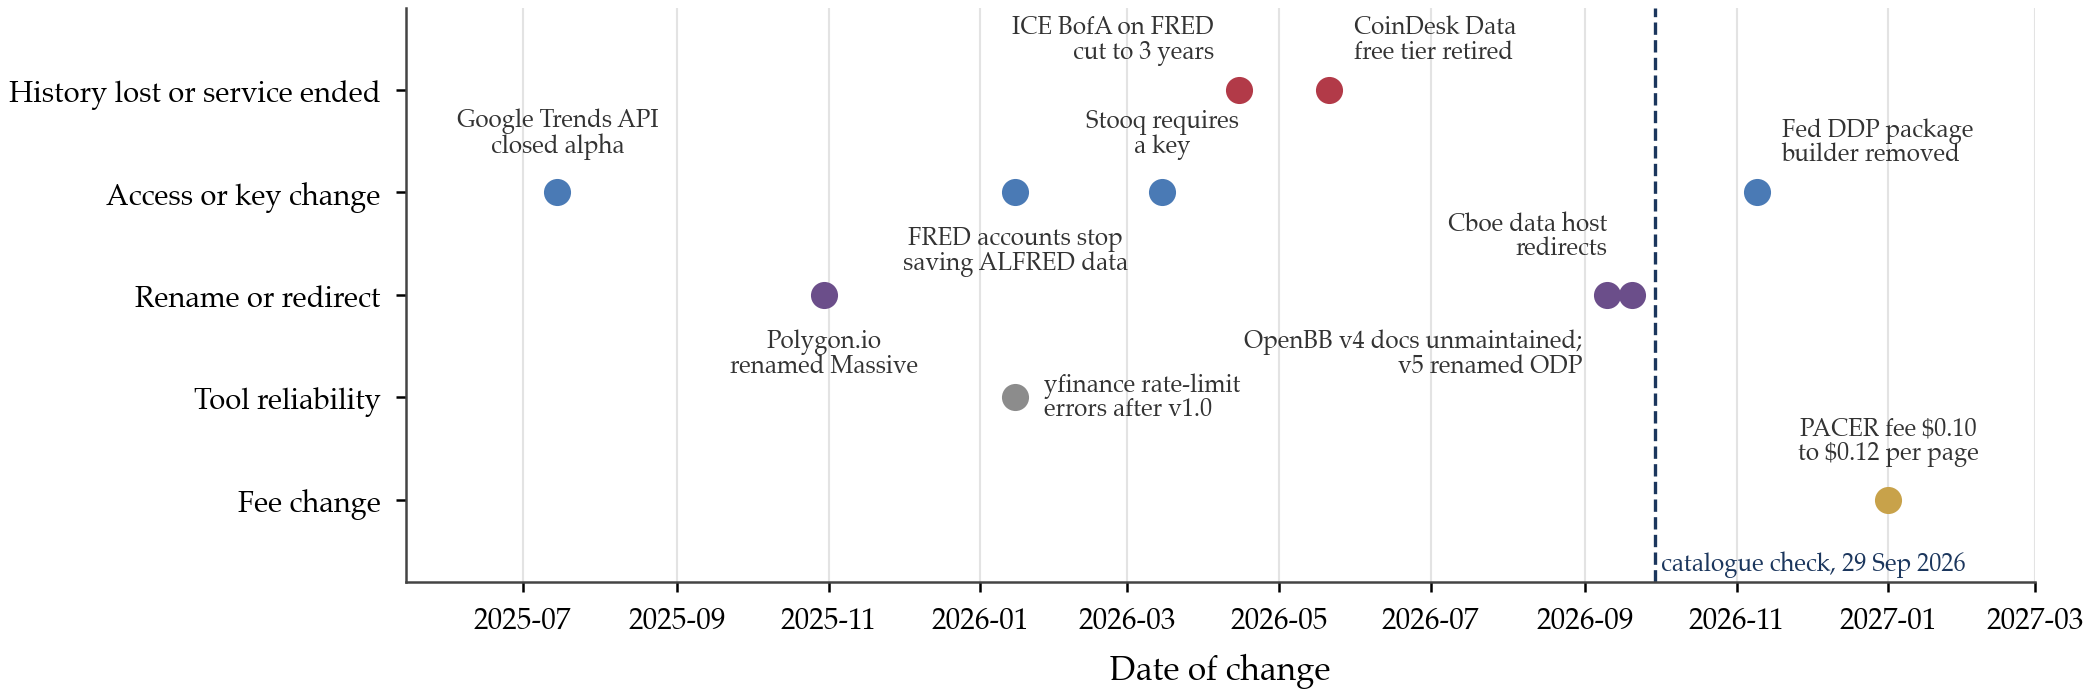
\includegraphics[width=\textwidth]{figures/changes_timeline.png}
\caption{Dated terms changes, shutdowns and renames recorded in the catalogue, July 2025 to January 2027, by type of change. Eleven of the sixteen timeline entries carry a month or a day; entries dated only to a month are plotted at mid-month. The dashed line marks the catalogue check of 29 September 2026; two entries post-date it (the Federal Reserve change of November 2026, and the PACER fee rise, announced in advance). Change types are the author's grouping.}
\label{fig:changes}
\qsource{Free-data catalogue, changes timeline; author's grouping by type.}
\end{figure*}

Three design rules follow from the earlier sections. First, every capture should store the retrieval time alongside the raw response, because for snapshot sources the retrieval time is the only point-in-time stamp there is. Second, a failed call or a changed schema should raise an alert rather than write an empty record, since a silent gap in an archive is indistinguishable from a quiet market. Third, licence terms travel with the data: an archive of internal-use series is itself for internal use.

The archive also has to survive change in the sources themselves. The catalogue's timeline of terms changes, shutdowns and renames from 2025 to 2027 has sixteen entries; Figure~\ref{fig:changes} places the eleven that carry a month or a day. Two removed history outright: the cut of the ICE BofA indices to three years in April 2026 and the end of the CryptoCompare free tier on 21 May 2026 \cite{coindesk}. Four changed access, among them Stooq's key requirement from March 2026, which broke a widely used Python reader, and the removal of the package builder of the Federal Reserve's Data Download Program in the week of 9 November 2026, after which Federal Reserve series should be taken from FRED or the release feeds. Three were renames or redirects, one concerned a tool's reliability (yfinance), and one is a fee rise: PACER moves from \$0.10 to \$0.12 per page on 1 January 2027 for five years, with the quarterly fee waiver rising from \$30 to \$40 \cite{unc}. Five entries carry no month: the Russell move to June and December reconstitutions in 2026 \cite{lseg}, and four standing changes (the EDGAR form codes, the CFTC contract names, the two-year OCC cap and Kalshi's split between live and historical endpoints).

%═══════════════════════════════════════════════════════
\section{Limitations}
\label{sec:limits}

The survey has five limitations. First, every check is a single observation on 29 September 2026. Endpoints, limits and terms change, as Section~\ref{sec:archive} shows, and any entry should be re-tested before it is relied on. Second, evidence quality is uneven: 17 of the 73 entries are reported from documentation alone, and the alternative-data area in particular rests mostly on such reports. The three-fold check was applied to the top 50 claims, not to every field of every entry. Third, many cells in Tables~\ref{tab:src-rates}--\ref{tab:src-macro} are blank because the catalogue does not state the history or the lag; these are gaps in the survey, not properties of the sources, and the lag column in particular should be measured before any backtest relies on it. Fourth, coverage is weighted toward U.S.\ markets and toward the strategy families the desk was considering; Section~\ref{sec:gaps} lists the areas not researched in depth. Fifth, the survey is about inputs. It contains no backtests, and no statement in it should be read as evidence that any strategy is profitable.

%═══════════════════════════════════════════════════════
\section{Conclusion}
\label{sec:conclusion}

For a small systematic desk, free public data is enough to start research in most of the strategy families surveyed. Official and exchange sources cover funding markets, Treasury supply, futures positioning, energy and agricultural fundamentals, volatility indices and corporate filings without charge, and many of them are the primary record. The constraints are of three kinds. Several of the most useful sources are snapshots or rolling windows, so the desk must archive them daily or lose their history; publication timing is often unstated, so each source needs an explicit availability date before it enters a backtest; and licence terms limit what can be published or sold. Where free data runs out (bulk bond trades, historical option surfaces, convertible terms, CDS, live borrow and futures settlement history), the survey identifies the specific products to buy. The practical order of work that follows is to build the archiver first, then the twelve priority feeds, and to measure every lag before using it.

%═══════════════════════════════════════════════════════
\section*{Catalogue Availability}

The full catalogue is maintained in this repository: every entry with its example endpoint, documentation link, limits and caveats, together with the 33 playbooks, the priority feeds, the archive list, the gaps table and the changes timeline. Endpoints change; re-test any entry before relying on it. No data are distributed with this paper.

%═══════════════════════════════════════════════════════
\begin{thebibliography}{99}
\small\raggedright

\bibitem{croushore2001}
D.~Croushore and T.~Stark.
\newblock ``A real-time data set for macroeconomists.''
\newblock \textit{Journal of Econometrics}, 105(1):111--130, 2001.

\bibitem{nyfed}
Federal Reserve Bank of New York.
\newblock Markets Data API documentation.
\newblock \url{https://markets.newyorkfed.org/static/docs/markets-api.html}.

\bibitem{ofr}
Office of Financial Research.
\newblock Short-term Funding Monitor API.
\newblock \url{https://www.financialresearch.gov/short-term-funding-monitor/api/}.

\bibitem{alfred}
Federal Reserve Bank of St.\ Louis.
\newblock FRED API: ALFRED vintage data documentation.
\newblock \url{https://fred.stlouisfed.org/docs/api/fred/alfred.html}.

\bibitem{fiscal}
U.S.\ Department of the Treasury, Bureau of the Fiscal Service.
\newblock Fiscal Data API documentation.
\newblock \url{https://fiscaldata.treasury.gov/api-documentation/}.

\bibitem{cftc}
Commodity Futures Trading Commission.
\newblock Public Reporting Environment (Commitments of Traders).
\newblock \url{https://publicreporting.cftc.gov/}.

\bibitem{cboe}
Cboe Global Markets.
\newblock VIX historical data; CFE historical market statistics.
\newblock \url{https://www.cboe.com/tradable_products/vix/vix_historical_data}.

\bibitem{occ}
The Options Clearing Corporation.
\newblock Market data reports.
\newblock \url{https://www.theocc.com/market-data/market-data-reports}.

\bibitem{sec}
U.S.\ Securities and Exchange Commission.
\newblock EDGAR application programming interfaces; fails-to-deliver data; Form 13F data sets.
\newblock \url{https://www.sec.gov/search-filings/edgar-application-programming-interfaces}.

\bibitem{finra}
FINRA.
\newblock TRACE data pricing; equity short interest data.
\newblock \url{https://www.finra.org/filing-reporting/trace/pricing}.

\bibitem{eia}
U.S.\ Energy Information Administration.
\newblock Open data (API v2) and Weekly Petroleum Status Report.
\newblock \url{https://www.eia.gov/opendata/}.

\bibitem{usda}
U.S.\ Department of Agriculture.
\newblock NASS Quick Stats API; FAS Production, Supply and Distribution Online.
\newblock \url{https://quickstats.nass.usda.gov/api}.

\bibitem{ftc}
Federal Trade Commission.
\newblock HSR early termination notices API.
\newblock \url{https://www.ftc.gov/developer/api/v0/endpoints/hsr-early-termination-notices}.

\bibitem{cl}
Free Law Project.
\newblock CourtListener REST API.
\newblock \url{https://www.courtlistener.com/help/api/rest/}.

\bibitem{unc}
University of North Carolina School of Law Library.
\newblock ``PACER alternatives and cost-cutting strategies in anticipation of fee increases.'' July 2026.

\bibitem{lseg}
LSEG.
\newblock ``FTSE Russell announces December 2026 Russell US indexes reconstitution schedule.'' Press release, 2026.

\bibitem{kalshi}
Kalshi.
\newblock Historical data documentation.
\newblock \url{https://docs.kalshi.com/getting_started/historical_data}.

\bibitem{poly}
Polymarket.
\newblock API rate limits.
\newblock \url{https://docs.polymarket.com/api-reference/rate-limits}.

\bibitem{deribit}
Deribit.
\newblock API documentation.
\newblock \url{https://docs.deribit.com/}.

\bibitem{gtrends}
Google Search Central.
\newblock Announcement of the Google Trends API (alpha). July 2025.
\newblock \url{https://developers.google.com/search/blog/2025/07/trends-api}.

\bibitem{coindesk}
CoinDesk Data.
\newblock ``Changes to CoinDesk Data indices API free tier access.'' 2026.

\end{thebibliography}

{\footnotesize\noindent Web resources were consulted for the catalogue check of 29 September 2026.\par}

%═══════════════════════════════════════════════════════
\onecolumn
\appendix
\renewcommand{\thetable}{A\arabic{table}}
\renewcommand{\theHtable}{A\arabic{table}}
\setcounter{table}{0}
\section{The Catalogue by Area}
\label{app:catalogue}

Tables~\ref{tab:src-rates}--\ref{tab:src-macro} list all 73 catalogue entries, grouped as in Section~\ref{sec:sources}. Access and evidence codes are as in Section~\ref{sec:method} (V verified, L live-tested, R reported); a dash means the catalogue does not state the item, not that it is absent; identifiers in brackets are those of Figure~\ref{fig:matrix}.

{\footnotesize
\setlength{\tabcolsep}{3.5pt}
\qstripes
\begin{longtable}{@{}L{3.1cm}L{4.65cm}L{1.85cm}L{2.5cm}L{2.7cm}L{1.35cm}@{}}
\caption{Rates, funding and credit (15 entries). Evidence: V verified, L live-tested, R reported. A dash means not stated in the catalogue.}\label{tab:src-rates}\\
\toprule
\qhead{Source (identifier)} & \qhead{What it provides} & \qhead{Frequency} & \qhead{Free history} & \qhead{Timing and lag} & \qhead{Access} \\
\midrule
\endfirsthead
\toprule
\qhead{Source (identifier)} & \qhead{What it provides} & \qhead{Frequency} & \qhead{Free history} & \qhead{Timing and lag} & \qhead{Access} \\
\midrule
\endhead
\bottomrule
\endfoot
\bottomrule
\hiderowcolors
\multicolumn{6}{@{}p{\textwidth}@{}}{\qsource{Free-data catalogue (rates, funding and credit entries), checked 29 September 2026; provider documentation \cite{nyfed,ofr,alfred,fiscal,cftc,finra}.}}
\endlastfoot
NY Fed Markets Data API (\sid{nyfed}) & SOFR, EFFR, OBFR, TGCR, BGCR with percentiles and volume; repo and reverse-repo operations; SOMA holdings by CUSIP; dealer statistics & Daily & EFFR before 2016 in a different schema & \ns & none, V \\
OFR Short-term Funding Monitor (\sid{ofr}) & About 442 series: money funds, repo by segment, reference rates, dealer statistics, Treasury yields; vintage selection & Daily to weekly & 10-year yield from 1990; dealer series from 2015 & \ns & none, V \\
FRED and ALFRED (\sid{fred}) & St.\ Louis Fed macro and market series, with every past vintage & By series & 10-year yield daily from 1962 & Vintages record what was known on each date & key, V \\
Treasury FiscalData (\sid{fiscal}) & Auction results; Daily Treasury Statement including the TGA balance & Per auction; daily & \ns & \ns & none, L \\
TreasuryDirect (\sid{tdirect}) & Announced and auctioned securities by CUSIP & Per auction & \ns & \ns & none, L \\
Treasury par yield curve (\sid{tcurve}) & Official daily par nominal curve & Daily & \ns & \ns & none, L \\
CFTC Commitments of Traders (\sid{cot}) & Positioning by trader class: legacy, disaggregated and financial-futures reports & Weekly & Futures only from 1986; with options from 1995 & Tuesday positions, released Friday 15:30 ET & none, L \\
Federal Reserve Board RSS (\sid{fedrss}) & FOMC statements and minutes, speeches, release notices, H.15/H.10 series feeds & On release & Series feeds hold the latest value only & Time stamp is the scheduled release time & none, V \\
ECB Data Portal (\sid{ecb}) & Euro-area government yield curves (spot, par, forward) & Daily & \ns & \ns & none, L \\
Bank of England Database (\sid{boe}) & Any BoE series by code, e.g.\ SONIA & Daily & \ns & \ns & none, L \\
BIS Data Portal (\sid{bis}) & Central-bank policy rates for dozens of countries & Daily & Long history (not dated) & \ns & none, L \\
Chatham Financial rates page (\sid{chatham}) & Current U.S.\ market rates including SOFR swap rates & Daily & Current page only & \ns & scrape, R \\
ICE BofA OAS on FRED (\sid{iceoas}) & Option-adjusted spreads: high yield, BBB, investment grade, AAA & Daily & Rolling 3 years since April 2026 & Close posted the next morning & none, V \\
FINRA TRACE (\sid{trace}) & Corporate, agency and Treasury bond trades; free site shows one bond at a time & Trade by trade & Free site: rolling 3 years & Bulk files quarterly, 6-month lag & paid, V \\
MSRB EMMA (\sid{emma}) & Municipal bond trade prices and issuer disclosures & Trade by trade & \ns & \ns & none, R \\
\end{longtable}
}

{\footnotesize
\setlength{\tabcolsep}{3.5pt}
\qstripes
\begin{longtable}{@{}L{3.1cm}L{4.65cm}L{1.85cm}L{2.5cm}L{2.7cm}L{1.35cm}@{}}
\caption{Commodities, weather and alternative data (17 entries).}\label{tab:src-commod}\\
\toprule
\qhead{Source (identifier)} & \qhead{What it provides} & \qhead{Frequency} & \qhead{Free history} & \qhead{Timing and lag} & \qhead{Access} \\
\midrule
\endfirsthead
\toprule
\qhead{Source (identifier)} & \qhead{What it provides} & \qhead{Frequency} & \qhead{Free history} & \qhead{Timing and lag} & \qhead{Access} \\
\midrule
\endhead
\bottomrule
\endfoot
\bottomrule
\hiderowcolors
\multicolumn{6}{@{}p{\textwidth}@{}}{\qsource{Free-data catalogue (commodities and alternative-data entries), checked 29 September 2026; provider documentation \cite{eia,usda,gtrends}.}}
\endlastfoot
EIA API v2 (\sid{eia}) & Petroleum, natural gas, power and coal, including weekly stocks and gas storage & Weekly to annual & \ns & No ``last updated'' field; track the release calendar & key, L \\
EIA weekly petroleum tables (\sid{wpsr}) & Weekly petroleum report tables as CSV: crude, SPR, gasoline, distillate & Weekly & \ns & \ns & none, L \\
EIA Daily Prices (\sid{eiaprices}) & Crack spread, spark spreads, spot gas at ten hubs, power hubs & Weekdays & \ns & 07:30--08:30 ET, prior-day closes & none, R \\
USDA NASS Quick Stats (\sid{nass}) & Crop progress and condition, acreage, yield, production, to county level & Weekly in season; monthly, annual & \ns & \ns & key, V \\
USDA FAS PSD Online (\sid{psd}) & Global supply-and-demand balance sheets by country & Monthly & From 1960 & Within 2 working days of WASDE & none, V \\
LBMA precious-metals prices (\sid{lbma}) & Gold price in USD, GBP and EUR & Daily & Gold PM from 1968 & \ns & none, L \\
NOAA CPC degree days (\sid{cpc}) & Population-weighted heating and cooling degree days by census division & Daily & \ns & \ns & none, L \\
UN Comtrade (\sid{comtrade}) & Bilateral trade flows by HS product code & Monthly & \ns & Lagged by country & none, L \\
JODI Oil (\sid{jodi}) & Oil production, demand and stocks by country & Monthly & \ns & \ns & none, R \\
CME Group website (\sid{cme}) & Futures and options settlements, volume, open interest (browser view) & Daily & Bulk history is paid & \ns & scrape, L \\
NOAA Climate Data Online (\sid{cdo}) & Station and regional climate summaries, storm events & Daily & \ns & \ns & key, R \\
Open-Meteo (\sid{openmeteo}) & Global weather forecasts by latitude and longitude & Through the day & Forecasts & \ns & none, L \\
ECMWF open data (\sid{ecmwf}) & Published forecast files (GRIB format) & Per model run & \ns & \ns & none, R \\
AISStream (\sid{ais}) & Real-time ship positions and static data over WebSocket & Real time & \ns & \ns & key, R \\
Drewry World Container Index (\sid{drewry}) & Container freight rate index & Weekly & \ns & \ns & scrape, R \\
Google Trends API (\sid{gtrends}) & Consistently scaled search interest by region & Daily to yearly & Rolling 5 years & Data to about 2 days ago & account, R \\
Reddit and StockTwits (\sid{social}) & Retail investor discussion & Real time & \ns & \ns & account, L \\
\end{longtable}
}

{\footnotesize
\setlength{\tabcolsep}{3.5pt}
\qstripes
\begin{longtable}{@{}L{3.1cm}L{4.65cm}L{1.85cm}L{2.5cm}L{2.7cm}L{1.35cm}@{}}
\caption{Volatility, options, crypto-assets and prediction markets (13 entries).}\label{tab:src-vol}\\
\toprule
\qhead{Source (identifier)} & \qhead{What it provides} & \qhead{Frequency} & \qhead{Free history} & \qhead{Timing and lag} & \qhead{Access} \\
\midrule
\endfirsthead
\toprule
\qhead{Source (identifier)} & \qhead{What it provides} & \qhead{Frequency} & \qhead{Free history} & \qhead{Timing and lag} & \qhead{Access} \\
\midrule
\endhead
\bottomrule
\endfoot
\bottomrule
\hiderowcolors
\multicolumn{6}{@{}p{\textwidth}@{}}{\qsource{Free-data catalogue (volatility, options, crypto and prediction-market entries), checked 29 September 2026; provider documentation \cite{cboe,occ,deribit,kalshi,poly,coindesk}.}}
\endlastfoot
Cboe volatility indices (\sid{cboeidx}) & VIX, VIX9D, VIX3M, VVIX, SKEW, COR3M, OVX, GVZ, VXAPL, VXAZN, VXEEM & Daily & VIX, SKEW from 1990; VVIX, COR3M 2006; VIX3M 2009 & \ns & none, V \\
Cboe delayed option chains (\sid{cboechain}) & Full chain: quotes, volume, open interest, Cboe IV and Greeks per contract & Snapshot & None (snapshot only) & Delayed; cached about 5 s & none, V \\
Cboe CFE futures data (\sid{cfe}) & Per-contract VIX and Mini-VIX futures files; volume and open interest for all CFE products & Daily & VIX futures from 2013; volume and open interest from 2004 & \ns & none, V \\
Cboe daily statistics (\sid{cboestats}) & Total, index, ETP and equity put/call ratios & Daily & \ns & \ns & none, L \\
OCC market data (\sid{occ}) & Cleared volume by customer, firm and market maker, calls and puts; open interest by strike & Daily, weekly, monthly & Rolling 2 years & \ns & none, V \\
SqueezeMetrics (\sid{squeeze}) & Dark-pool index (DIX) and estimated dealer gamma exposure (GEX) for the S\&P~500 & Daily & From May 2011 & \ns & none, V \\
Nasdaq calendars (\sid{nasdaqcal}) & Earnings dates with consensus EPS; dividend ex, record and pay dates & Daily & \ns & \ns & none, L \\
yfinance (\sid{yf}) & Unofficial Yahoo Finance prices, fundamentals and option chains & End of day; delayed intraday & \ns & \ns & none, R \\
Deribit public API (\sid{deribit}) & All BTC and ETH options with IV and open interest; DVOL; trades; funding & Real time & DVOL history; hourly realised volatility about 16 days & \ns & none, V \\
Binance futures API (\sid{binance}) & Mark and index prices, funding rates; bulk archives & Real time; funding 8-hourly & Bulk archives & \ns & none, L \\
CoinDesk Data, ex-CryptoCompare (\sid{coindesk}) & Multi-exchange crypto-asset data & \ns & Free tier ended 21 May 2026 & \ns & paid, R \\
Kalshi API (\sid{kalshi}) & Prices for CFTC-regulated event contracts & Real time & Older data moves to separate historical endpoints & \ns & none, L \\
Polymarket APIs (\sid{poly}) & Market metadata, prices, order books, price history & Real time & Price history & \ns & none, L \\
\end{longtable}
}

{\footnotesize
\setlength{\tabcolsep}{3.5pt}
\qstripes
\begin{longtable}{@{}L{3.1cm}L{4.65cm}L{1.85cm}L{2.5cm}L{2.7cm}L{1.35cm}@{}}
\caption{Filings, news, event-driven situations and funds (22 entries).}\label{tab:src-event}\\
\toprule
\qhead{Source (identifier)} & \qhead{What it provides} & \qhead{Frequency} & \qhead{Free history} & \qhead{Timing and lag} & \qhead{Access} \\
\midrule
\endfirsthead
\toprule
\qhead{Source (identifier)} & \qhead{What it provides} & \qhead{Frequency} & \qhead{Free history} & \qhead{Timing and lag} & \qhead{Access} \\
\midrule
\endhead
\bottomrule
\endfoot
\bottomrule
\hiderowcolors
\multicolumn{6}{@{}p{\textwidth}@{}}{\qsource{Free-data catalogue (filings, news, event-driven and fund entries), checked 29 September 2026; provider documentation \cite{sec,finra,ftc,cl,unc,lseg}.}}
\endlastfoot
SEC EDGAR APIs (\sid{edgar}) & Company submissions and XBRL financials; nightly bulk files & Real time & \ns & Submissions under 1 s; XBRL under 1 minute & none, V \\
EDGAR latest filings feed (\sid{edgarfeed}) & Newest filings by form type & 06:00--22:00 ET, business days & \ns & \ns & none, L \\
EDGAR full-text search (\sid{efts}) & Search of filing text with form and date filters & Near real time & \ns & \ns & none, L \\
SEC Form 13F data sets (\sid{f13}) & Structured institutional holdings as filed & Quarterly & From 2013 Q2 & Released after end of Feb, May, Aug, Nov & none, R \\
SEC fails-to-deliver (\sid{ftd}) & Cumulative settlement fails by CUSIP & Twice monthly & Before Sep 2008, fails of 10,000+ shares only & 2--6 weeks & none, V \\
FINRA short interest (\sid{finrasi}) & Short interest, days to cover, average volume, listed and OTC stocks & Twice monthly & Before June 2021, OTC stocks only & \ns & none, V \\
Interactive Brokers shortable file (\sid{ibkr}) & Indicative borrow fee, rebate and shares available, by country & Through the day & None (snapshot only) & \ns & none, V \\
Federal Register API (\sid{fedreg}) & Rules, proposed rules and notices of federal agencies & Daily & \ns & \ns & none, L \\
ECB and BoE RSS (\sid{cbrss}) & Central-bank press releases & On release & \ns & \ns & none, L \\
GlobeNewswire RSS (\sid{gnw}) & Press releases by subject, including M\&A & Real time & \ns & \ns & none, L \\
GDELT (\sid{gdelt}) & Machine-coded global news events; article search & Every 15 minutes & Archive to 1979 & \ns & none, L \\
FTC HSR early termination (\sid{ftc}) & Deals granted early termination of the HSR waiting period (not expiries or second requests) & Roughly weekly & \ns & \ns & key, V \\
UK CMA merger cases (\sid{cma}) & Merger case records via the GOV.UK search API & As cases update & \ns & \ns & none, L \\
EU competition cases (\sid{eucomp}) & EU merger case search & As cases update & \ns & \ns & scrape, R \\
CourtListener RECAP (\sid{cl}) & Federal dockets including bankruptcy & Continuous & Only documents already bought on PACER & \ns & none, L \\
PACER (\sid{pacer}) & Official federal court dockets and documents & Real time & \ns & \ns & paid, R \\
Delaware claims agents (\sid{deb}) & About 269 cases with bar dates and claims agents (probably a subset) & As cases file & \ns & \ns & none, V \\
FTSE Russell reconstitution (\sid{russell}) & Russell U.S.\ index reconstitution schedules & June and December & \ns & Dated rank day, lists, lock-down, effective date & none, V \\
S\&P Dow Jones Indices (\sid{spdji}) & Index change announcements & As announced & \ns & \ns & scrape, L \\
CEF Connect (\sid{cef}) & Closed-end fund price, NAV and discount & Daily & \ns & \ns & none, L \\
ETF issuer holdings files (\sid{ssga}) & Daily holdings per ETF (SPDR files tested) & Daily & \ns & \ns & none, L \\
Artemis (\sid{artemis}) & Catastrophe-bond and insurance-linked securities deal directory & As deals issue & Directory since the mid-1990s & \ns & scrape, R \\
\end{longtable}
}

{\footnotesize
\setlength{\tabcolsep}{3.5pt}
\qstripes
\begin{longtable}{@{}L{3.1cm}L{4.65cm}L{1.85cm}L{2.5cm}L{2.7cm}L{1.35cm}@{}}
\caption{Macro and general market data (6 entries).}\label{tab:src-macro}\\
\toprule
\qhead{Source (identifier)} & \qhead{What it provides} & \qhead{Frequency} & \qhead{Free history} & \qhead{Timing and lag} & \qhead{Access} \\
\midrule
\endfirsthead
\toprule
\qhead{Source (identifier)} & \qhead{What it provides} & \qhead{Frequency} & \qhead{Free history} & \qhead{Timing and lag} & \qhead{Access} \\
\midrule
\endhead
\bottomrule
\endfoot
\bottomrule
\hiderowcolors
\multicolumn{6}{@{}p{\textwidth}@{}}{\qsource{Free-data catalogue (macro and general market-data entries), checked 29 September 2026.}}
\endlastfoot
IMF, OECD and World Bank (\sid{imf}) & Cross-country macro data (SDMX and REST interfaces) & Monthly to annual & \ns & \ns & none, L \\
BLS API and calendar (\sid{bls}) & CPI, payrolls and other series; calendar of scheduled releases & Monthly & \ns & Calendar covers the year ahead & none, L \\
Alpha Vantage (\sid{av}) & Market and economic data, including Treasury yields & Daily & \ns & \ns & key, L \\
Nasdaq Data Link (\sid{ndl}) & Data sets formerly under Quandl & Varies & \ns & \ns & key, L \\
Stooq (\sid{stooq}) & Daily prices for global equities, indices, FX and futures & Daily & Long daily history (not dated) & \ns & key, R \\
Massive, ex-Polygon.io (\sid{massive}) & Market data with a free tier & Varies & \ns & \ns & key, R \\
\end{longtable}
}

\end{document}
